\documentclass{beamer}
%%% plots %%%
%%% table%%%
%%% plots %%%
\usepackage{relsize}
\newcommand{\bigqm}[1][1]{\text{\larger[#1]{\textbf{?}}}}
\usepackage{pgfplots,filecontents}
\pgfplotsset{compat=1.7}
\usetikzlibrary{backgrounds}
\tikzset{
	circ/.style={circle, fill=black, inner sep=2pt, node contents={}}
}
\tikzset{
	block/.style = {draw, fill=white!50, thick, minimum width=1.7cm, minimum height=1.2cm, node distance=3cm},
	down/.style={yshift=-7em},
	up/.style={yshift=7em},
	right/.style={xshift=15em},
	downright/.style={xshift=12em, yshift = -7em},
	downleft/.style={xshift=-12em, yshift = -7em}
}
\usepackage{makecell}
\usetikzlibrary{shapes}
\usetikzlibrary{shapes.arrows}
\tikzset{
	myarrow/.style={
		draw,
		fill=black,
		single arrow,
		minimum height=3.5ex,
		single arrow head extend=1ex
	}
}
\newcommand{\arrowup}{%
	\tikz [baseline=-0.5ex]{\node [myarrow,rotate=90] {};}
}
\newcommand{\arrowdown}{%
	\tikz [baseline=-1ex]{\node [myarrow,rotate=-90] {};}
}
\newcommand{\arrowright}{%
	\tikz [baseline=-0.5ex]{\node [myarrow,rotate=0] {};}
}
\newcommand{\arrowleft}{%
	\tikz [baseline=-1ex]{\node [myarrow,rotate=-180] {};}
}
\usetikzlibrary{shapes.geometric}
\usetikzlibrary{calc}
\usetikzlibrary{arrows}
\usepackage{verbatim}
\def\foldedpaper#1{
	\tikz[scale=#1,line width={#1*1pt}]{
		\def\a{1.41} % relative height
		\def\b{0.2}  % relative height/width of corner
		\def\c{0.1}  % relative margin width (on either side)
		\def\d{0.05} % vertical offset of lines
		\def\N{6}    % number of lines
		\draw         (0,0)
		--  ++(-1,0)
		--  ++(0,\a)
		--  ++(1-\b,0)
		--  ++(\b,-\b)
		-- cycle;
		\foreach \lnum in {1,...,\N}{
			\pgfmathsetmacro\yline{\a-\d-\lnum*\a/(\N+1)}
			\draw (-1+\c,\yline) -- (-\c,\yline);
		}
		\draw[fill=white] (0,\a-\b) -- ++(-\b,0) -- ++ (0,\b);
	}
}


\def\man#1;{%
	\begin{scope}[shift={#1}]
		\fill [rounded corners=1.5] (0,0.4) -- (0,0.8) -- (0.4,0.8) -- (0.4,0.4) --
		(0.325,0.4) -- (0.325,0.7) -- (0.3,0.7) -- (0.3,0) -- (0.225,0) --
		(0.225,0.4) -- (0.175,0.4) -- (0.175,0) -- (0.1,0) -- (0.1,0.7) --
		(0.075,0.7) -- (0.075,0.4) -- cycle;
		\fill (0.2,0.9) circle (0.1);
	\end{scope}}
	\def\shadecircle(#1)(#2);{%
		\draw [thick] (#1) circle (#2);
		\draw [thick,draw opacity=0.1] (#1) ++(0,-0.1) circle (#2);}
	
	\tikzstyle{decision} = [diamond, draw,fill=white!50, 
	text width=4.5em, text badly centered, node distance=3cm, inner sep=0pt]
	\tikzstyle{block_flow} = [rectangle, draw, fill=white!50, 
	text centered, rounded corners, minimum height=4em]
	\tikzstyle{line} = [draw, -latex']
	\tikzstyle{cloud} = [draw, ellipse, node distance=3cm,
	minimum height=2em]
	
	
	\makeatletter
	\tikzset{
		through point/.style={
			to path={%
				\pgfextra{%
					\tikz@scan@one@point\pgfutil@firstofone(\tikztostart)\relax
					\pgfmathsetmacro{\pt@sx}{\pgf@x * 0.03514598035}%
					\pgfmathsetmacro{\pt@sy}{\pgf@y * 0.03514598035}%
					\tikz@scan@one@point\pgfutil@firstofone#1\relax
					\pgfmathsetmacro{\pt@ax}{\pgf@x * 0.03514598035 - \pt@sx}%
					@firstofone(\tikztota				\pgfmathsetmacro{\pt@ay}{\pgf@y * 0.03514598035 - \pt@sy}%
					\tikz@scan@one@point\pgfutilrget)\relax
					\pgfmathsetmacro{\pt@ex}{\pgf@x * 0.03514598035 - \pt@sx}%
					\pgfmathsetmacro{\pt@ey}{\pgf@y * 0.03514598035 - \pt@sy}%
					\pgfmathsetmacro{\pt@len}{\pt@ex * \pt@ex + \pt@ey * \pt@ey}%
					\pgfmathsetmacro{\pt@t}{(\pt@ax * \pt@ex + \pt@ay * \pt@ey)/\pt@len}%
					\pgfmathsetmacro{\pt@t}{(\pt@t > .5 ? 1 - \pt@t : \pt@t)}%
					\pgfmathsetmacro{\pt@h}{(\pt@ax * \pt@ey - \pt@ay * \pt@ex)/\pt@len}%
					\pgfmathsetmacro{\pt@y}{\pt@h/(3 * \pt@t * (1 - \pt@t))}%
				}
				(\tikztostart) .. controls +(\pt@t * \pt@ex + \pt@y * \pt@ey, \pt@t * \pt@ey - \pt@y * \pt@ex) and +(-\pt@t * \pt@ex + \pt@y * \pt@ey, -\pt@t * \pt@ey - \pt@y * \pt@ex) .. (\tikztotarget)
			}
		}
	}
	
	\makeatother
	
\usepackage{FiraSans}
\usetheme{metropolis} 
\usepackage{xgreek}
\usepackage [autostyle, english = american]{csquotes}
\MakeOuterQuote{"}
\usepackage{upgreek}
\title{Automated Data Scientist}
\date{
	\vspace{0.7cm}
	\begin{tabular}{ll} 
		 Εκπόνηση & Ελένη Νησιώτη \\
		 Επίβλεψη & Επίκ. Καθ. Ανδρέας Συμεωνίδης \\
		 Συνεπίβλεψη & Δρ. Κυριάκος Χατζηδημητρίου 
	\end{tabular}
	\\
	\\
	\\
	\\
	\\
	{ 
		 	\tiny \setlength{\parskip}{0.1em} 
		 \begin{tabular}{l}Αριστοτέλειο Πανεπιστήμιο Θεσσαλονίκης \\
		 	Πολυτεχνική Σχολή\\
		 	Τμήμα Ηλεκτρολόγων Μηχανικών και Μηχανικών Υπολογιστών\\
		 	Εργαστήριο Επεξεργασίας Πληροφορίας και Υπολογισμών 
		 \end{tabular}}}
\setlength{\parskip}{\baselineskip}%
\usepackage{graphicx}
\graphicspath{{./images/}}
\usepackage[backend=biber]{biblatex}
\addbibresource{bibliography.bib}
\begin{document}
  \maketitle
  \section{Σκοπός διπλωματικής εργασίας}
  \begin{frame}{Προβληματισμός}
  		\begin{flushleft}
  			{\small \textit 
  			To $ 75 \% $ ενός πειράματος μηχανικής μάθησης αφιερώνεται στην προετοιμασία της εφαρμογής του αλγορίθμου και το $15 \% $ στα βήματα που την ακολουθούν. Το μεγαλύτερο μέρος της έρευνας επικεντρώνεται στο ενδιάμεσο $10 \%$ \ldots }
  		\end{flushleft}
  		\rightline{{ --- Rich Caruana, ICML 2015}}
  		\begin{center}
  			\arrowdown
  		\end{center}
  		
  		Ανάγκη για \alert{επέκταση} της τρέχουσας έρευνας σε \alert{χρονοβόρα} στάδια της διαδικασίας εφαρμογής μηχανικής μάθησης που μέχρι τώρα γίνονταν \alert{χειροκίνητα}.
 \end{frame}
  \begin{frame}{Η εξέλιξη των προβλημάτων}
  	\begin{figure}[t]
  		\resizebox*{0.8\textwidth}{0.5\textheight}{
  		\includegraphics[width=\textwidth]{evolution}}
  	\end{figure}  
  	\begin{center}
  	\begin{minipage}{0.3\textwidth}
  		Απαιτητικότητα προβλημάτων
  	\end{minipage}\qquad
  	\begin{minipage}{0.1\textwidth}
       \arrowright       
       
       \arrowleft
  	\end{minipage}\qquad
  	\begin{minipage}{0.3\textwidth}
       Εμπλεκόμενη τεχνολογία
  	\end{minipage}
  	\end{center}
  \end{frame}
  \begin{frame}{Η εξέλιξη του ML}
  	\begin{flushleft}
  			{\small \textit 
  			Ο προγραμματισμός στοχεύει στην αυτοματοποίηση, η μηχανική μάθηση στην αυτοματοποίηση της αυτοματοποίησης και η αυτοματοποιημένη μηχανική μάθηση στην αυτοματοποίηση του να αυτοματοποιείς την αυτοματοποίηση.}
  	\end{flushleft}
  	\rightline{{--- Matthew Mayo, KDnuggets 2017 }}
  		\begin{center}
  			\arrowdown
  		\end{center}
  	Το \alert{νέο στάδιο} στην εξέλιξη της μηχανικής μάθησης στοχεύει στη δημιουργία \alert{μετα-γνώσης} για την αυτοματοποίηση της ίδιας της διαδικασίας της μάθησης και όχι μεμονωμένων προβλημάτων.
  	\end{frame}  
  \begin{frame}{Η επιστήμη του Automl}
  	\begin{minipage}[t]{.4\textwidth}  		
  		Απαρχές
  		\vspace{4ex}
  	\end{minipage}% This must go next to `\end{minipage}` \hspace{2cm}
  	  	\begin{minipage}[t]{.5\textwidth}
  	  		Unica, MarketSwitch, KXEN  	
  	  		\vspace{4ex}
  	  	\end{minipage}
  	\begin{minipage}[t]{.4\textwidth}  		
  		Πεδία Εφαρμογής
  		\vspace{4ex}
  	\end{minipage}% This must go next to `\end{minipage}` \hspace{2cm}
  	\begin{minipage}[t]{.5\textwidth}
  		Προ-επεξεργασία, Επιλογή αλγορίθμου, Ρύθμιση μοντέλου
  		\vspace{4ex} 
  	\end{minipage}
  	\begin{minipage}[t]{.4\textwidth}  		
  		Σύγχρονα Εργαλεία
  		\vspace{4ex}
  	\end{minipage}% This must go next to `\end{minipage}` \hspace{2cm}
	\begin{minipage}[t]{.5\textwidth}
  		AutoWeka, Microsoft Azure, caret, HPOlib, Google Automl
  		\vspace{4ex}
  	\end{minipage}
  \end{frame}
  
  \begin{frame} {Προτεινόμενο σύστημα}
  	Ένας \alert{αυτοματοποιημένος} αναλυτής δεδομένων για προβλήματα δυαδικής ταξινόμησης με \alert{εμπειρία} παλαιότερων πειραμάτων και \alert{κατανοητή} έξοδο.
  	\begin{center}
  		\arrowdown
  	\end{center}
  	\begin{itemize}
  		\item Αυτόματος σχηματισμός βέλτιστου ensemble
  		\item Ενσωμάτωση μετα-μάθησης
  		\item Παραγωγή επεξηγηματικού report για το χρήστη
  	\end{itemize}
  \end{frame}
  \section{Μεθοδολογία}
  \begin{frame} {No free lunch theorem}
  	\begin{flushleft}
  		{\small \textit 
  	    Αν λάβουμε υπόψιν όλες τις πιθανές κατανομές δημιουργίας δεδομένων, τότε κάθε αλγόριθμος μηχανικής μάθησης επιδεικνύει κατά μέσο όρο το ίδιο σφάλμα στην πρόβλεψη άγνωστων παραδειγμάτων.}
  	\end{flushleft}
  	\rightline{{--- David Wolpert, 1996}}  	
  	\begin{center}
  		\arrowdown
  	\end{center}  	
  	Είναι \alert{αδύνατη} η εύρεση ενός \alert{γενικά βέλτιστου αλγορίθμου}. Ένα εργαλείο βελτιστοποίησης γενικής φύσης προβλημάτων οφείλει να \alert{εξερευνήσει} το χώρο των πιθανών μηχανισμών δημιουργίας δεδομένων και να προσφέρει \alert{προσαρμοσμένες λύσεις}.
  \end{frame}
    \begin{frame} {Ρύθμιση μοντέλου: σύγχρονες τεχνικές βελτιστοποίησης}
    	\begin{center}
    	\begin{minipage}[t]{0.28\textwidth}
    		\begin{center}
    		\textbf{Πλεγματική} 
    		
    		\vspace{1cm}
    		χρονοβόρα
    		
    		\vspace{0.5cm}
    		ισοπίθανη αντιμετώπιση
    		\end{center}
    	\end{minipage}%
    	\begin{minipage}[t]{0.28\textwidth}
    		\begin{center}
    		\textbf{Τυχαία} 
    		
    		\vspace{1cm}
    		naive
    	\end{center}
    	\end{minipage}%
    	\begin{minipage}[t]{0.28\textwidth}
    		\begin{center}
    		\textbf{Bayesian} 
    		
    		\vspace{1cm}
    		χρονοβόρα
    		
    		\vspace{0.5cm}
    		intuitive
    	\end{center}
    	\end{minipage}    	
    	    \end{center}	
    \end{frame}
    \begin{frame} {Ρύθμιση μοντέλου: επισκόπηση}
    Οι σύγχρονες τεχνικές:
    \begin{itemize}
    	\item είναι χρονοβόρες
    	\item δεν μπορεί να αποδειχθούν γενικά βέλτιστες
    	\item είναι ad-hoc
    \end{itemize}
    \end{frame}
  \begin{frame}{Μετα-μάθηση}
  	\begin{minipage}[t]{.3\textwidth}  		
  		Σκοπός
  		\vspace{4ex}
  	\end{minipage}% This must go next to `\end{itemize}}` \hspace{2cm}
  	\begin{minipage}[t]{.6\textwidth}
  		Δημιουργία μετα-γνώσης από πειράματα μηχανικής μάθησης  	
  		\vspace{4ex}
  	\end{minipage}
  	\begin{minipage}[t]{.3\textwidth}  		
  		Τρόπος
  		\vspace{4ex}
  	\end{minipage}% This must go next to `\end{minipage}` \hspace{2cm}
  	\begin{minipage}[t]{.6\textwidth}
  		Εξαγωγή μετα-χαρακτηριστικών των σετ δεδομένων, τα οποία περιέχουν ουσιώδη πληροφορία
  		\vspace{4ex} 
  	\end{minipage}
  	\begin{minipage}[t]{.3\textwidth}  		
  		Εφαρμογές
  		\vspace{4ex}
  	\end{minipage}% This must go next to `\end{minipage}` \hspace{2cm}
  	\begin{minipage}[t]{.6\textwidth}
  		Πρόβλεψη βέλτιστου αλγορίθμου, υπερ-παραμέτρων 
  		\vspace{4ex}
  	\end{minipage}
  	\end{frame}
\begin{frame}{Mετα-χαρακτηριστικά}
\centering
\begin{table}
	\caption{Λίστα μετα-χαρακτηριστικών μετά από εφαρμογή φιλτραρίσματος}
	\label{table:meta2}
	\scalebox{0.65}{
			\begin{tabular}{|l|l|}
				\hline
				Άθροισμα αθροισμάτων & Τυπική απόκλιση επιπέδων    \\
				Άθροισμα μέγιστων τιμών &  Κυρτότητα επιπέδων  \\
				Μέση τιμή τυπικών αποκλίσεων  & Λοξότητα επιπέδων    \\
				Μέση τιμή ελαχίστων τιμών &  Πλήθος χαρακτηριστικών  \\
				Μέση τιμή κυρτοτήτων &   Λογάριθμος πλήθους χαρακτηριστικών \\
				Μέση τιμή λοξοτήτων &    Πλήθος παραδειγμάτων\\
				Τυπική απόκλιση ελαχίστων τιμών & Λογάριθμος πλήθους παραδειγμάτων   \\
				Ελάχιστη τιμή μέσων τιμών &  Ποσοστό αγνώστων τιμών  \\
				Ελάχιστη τιμή τυπικών αποκλίσεων &  Πλήθος αριθμητικών χαρακτηριστικών  \\
				Ελάχιστη τιμή ελαχίστων τιμών &  Πλήθος κατηγορικών χαρακτηριστικών  \\
				Ελάχιστη τιμή μεγίστων τιμών &  Μέγιστη πιθανότητα κλάσης    \\
				Ελάχιστη τιμή λοξοτήτων & Μέση τιμή πιθανοτήτων κλάσης   \\
				Κυρτότητα ελαχίστων τιμών & Ποσοστό {PC} για $95\%$ διακύμανση  \\
				Κυρτότητα μεγίστων τιμών & Κυρτότητα πρώτης {PC}   \\
				Λοξότητα λοξοτήτων & Λοξότητα {PC}   \\
				Άθροισμα επιπέδων &    \\
				\hline
			\end{tabular}}
\end{table}
\end{frame}
  \begin{frame}{Ensembles}
  	\begin{flushleft}
  		{\small \textit 
  			Μεταξύ ανταγωνιζομένων υποθέσεων πρέπει να επιλέγεται η απλούστερη.}
  	\end{flushleft}
  	\rightline{{--- Το ξυράφι του Occam}}

  	\begin{flushleft}
  		{\small \textit 
  			Ο συνδυασμός σωστών λύσεων σε ένα πρόβλημα, δε μπορεί παρά να λύνει το πρόβλημα τουλάχιστον εξίσου καλά.}
  	\end{flushleft}
  	\rightline{{--- Επίκουρος}}  	
  	\begin{flushleft}
  		{\small \textit 
  			Μία αναγκαία και ικανή συνθήκη για να είναι μία συλλογή μοντέλων πιο ακριβής από τα μοντέλα που την απαρτίζουν είναι αυτά να είναι ακριβή και ετερογενή.}
  	\end{flushleft}
  	\rightline{{ --- Dietterich}}
  \end{frame}
   \begin{frame}{Ensembles από αποθήκες μοντέλων}
   	\begin{minipage}[t]{.3\textwidth}  		
   		Πρόβλημα
   		\vspace{4ex}
   	\end{minipage}% This must go next to `\end{minipage}` \hspace{2cm}
   	\begin{minipage}[t]{.6\textwidth}
   		Παρουσία πολλών, ετερογενών και ενδεχομένως κακής ποιότητας μοντέλων 	
   		\vspace{4ex}
   	\end{minipage}
   	\begin{minipage}[t]{.3\textwidth}  		
   		Στόχος
   		\vspace{4ex}
   	\end{minipage}% This must go next to `\end{minipage}` \hspace{2cm}
   	\begin{minipage}[t]{.6\textwidth}  
   		Υπολογιστικά εφικτή τεχνική σχηματισμού συλλογής των αποδοτικότερων μοντέλων με αποφυγή υπερ-προσαρμογής 		
   		\vspace{4ex} 
   	\end{minipage}
   \end{frame}
   \begin{frame} {Ensemble με προς τα εμπρός επιλογή μοντέλων}
   	\begin{figure}[!htb]
   		\scalebox{0.7}{
   		\begin{tikzpicture}[node distance = 3cm]
   		% Place nodes
   		\node [block_flow] (gather) {\makecell{Συγκέντρωση \\μοντέλων}};
   		\node [block_flow, right of=gather] (init) {\makecell{Αρχικοποίηση\\ συλλογής\\ με Ν μοντέλα}};
   		\node [block_flow, right of=init] (sample) {\makecell{Δειγματοληψία \\ με\\ αντικατάσταση}};
   		\node [block_flow, align = center, right of=sample, xshift = -0.2cm] (eval) {\makecell{Αξιολόγηση\\μοντέλων\\δείγματος}};
   		\node [block_flow, align = center, right of=eval, xshift = -0.5cm] (add) {\makecell{Προσθήκη \\ καλύτερου\\ μοντέλου}};
   		\node [decision, right of=add, scale = 0.8, xshift = -1.2cm] (decide) {OK?};
   		% Draw edges
   		\path [line] (gather) -- (init);
   		\path [line] (init) -- (sample);
   		\path [line] (sample) -- (eval);
   		\path [line] (eval) -- (add);
   		\path [line] (add) -- (decide);
   		\path[line] (decide.south)  node [anchor=west] {\small OXI} |- ([xshift=-0.5cm,yshift=-0.5cm]add.south west) -|  
   		($(init)!.5!(sample)$); 
   		% additional 
   		\node[draw, fill=white!50,circle,minimum size=1cm,inner sep=0pt, above of =init,yshift=-1.5cm ] {$A$};
   		\node[draw, fill=white!50,circle,minimum size=1cm,inner sep=0pt, above of =sample,yshift=-1.5cm ] {$B$};
   		\end{tikzpicture}}
   	\end{figure}
   	A: αποφυγή υπερ-προσαρμογής σε μικρές αποθήκες
   	
   	Β: αποφυγή υπερ-προσαρμογής σε μεγάλες αποθήκες και αναγκαστικής συμπερίληψης κακών μοντέλων
   	\end{frame}
   	 \section{Αρχιτεκτονική Συστήματος}
   	 \begin{frame}{Υποσύστημα εκπαίδευσης}
   	 	\begin{figure}[!htb]
   	 		Σκοπός: {\small Εκπαίδευση HyperParameterPrediction (HPP) μοντέλων\\ } 
   	 		\vspace{0.5cm}    	
   	 		\resizebox{\textwidth}{0.45\textheight}{
   	 			\begin{tikzpicture}	[database/.style={
   	 				cylinder,
   	 				cylinder uses custom fill,
   	 				cylinder body fill=white!50,
   	 				cylinder end fill=white!50,
   	 				shape border rotate=90,
   	 				aspect=0.5,
   	 				draw
   	 			}]
   	 			\node[database] (db) at (0, -0.25cm) {\makecell{Αποθήκη \\datasets}};
   	 			\node[block, align = center, text width=2.5cm, text centered, minimum width = 2 cm] (A) at (2.5cm,1.5) {optimizer};
   	 			\node[block, align = center, text width=2.5cm, text centered, minimum width = 2 cm] (B) at (2.5cm,-1.5) {mfExtractor};	
   	 			\node[database, aspect = 0.2] (mfdb) at (6cm,-0.25cm) {\makecell{Αποθήκη \\μετα-δεδομένων}};	
   	 			\node[block, align = center, text width=2.5cm, text centered, minimum width = 2 cm] (C) at (9.5cm, -0.25cm) {metaLearner};
   	 			\node[database] (model)  at (13cm, -0.25cm) {HPP-Μοντέλο};	
   	 			\draw[->, thick] (db) |- (A);
   	 			\draw[->, thick] (db) |- (B);
   	 			\draw[->, thick] (A) -| (mfdb.north);
   	 			\draw[->, thick] (B) -| (mfdb.south);
   	 			\draw[->, thick] (mfdb) to (C);
   	 			\draw[->, thick] (C) to (model.west);
   	 			\end{tikzpicture}}
   	 	\end{figure}
   	 	\begin{center}
   	 		\begin{enumerate}
   	 			\item optimizer: Bελτιστοποίηση υπερ-παραμέτρων
   	 			\item mfExtractor: Eξαγωγή μετα-χαρακτηριστικών
   	 			\item metaLearner: Eκπαίδευση HPP μοντέλων
   	 		\end{enumerate}
   	 	\end{center}
   	 \end{frame}
   	 \begin{frame}{Υποσύστημα πειράματος}  
   	 	\begin{figure}
   	 		Σκοπός: {\small Παραγωγή βέλτιστου ensemble για δεδομένο πρόβλημα\\ }  
   	 		\vspace{0.5cm}
   	 		\resizebox{\textwidth}{0.45\textheight}{
   	 			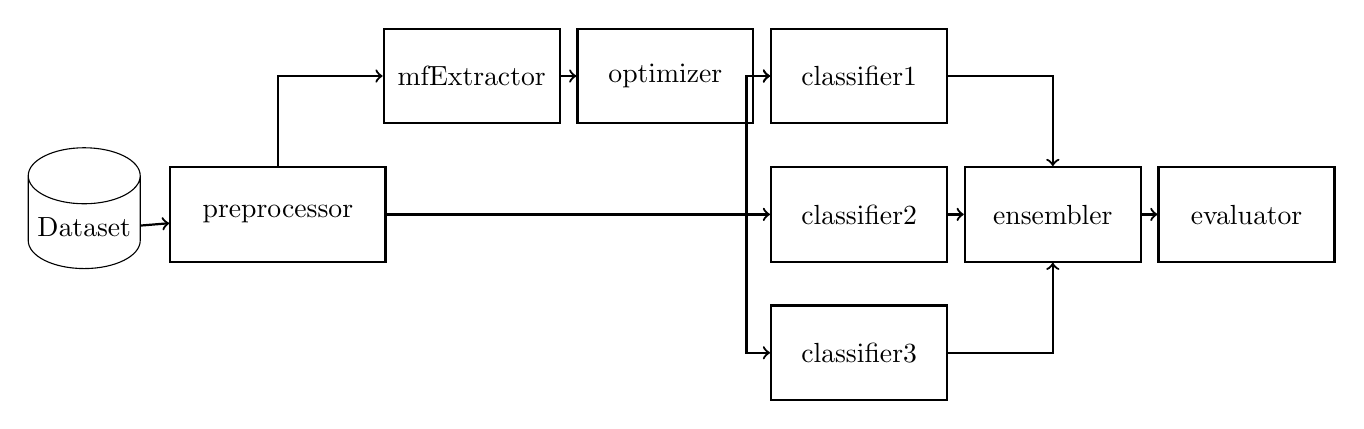
\begin{tikzpicture}	[database/.style={
   	 				cylinder,
   	 				cylinder uses custom fill,
   	 				cylinder body fill=white!50,
   	 				cylinder end fill=white!50,
   	 				shape border rotate=90,
   	 				aspect=0.5,
   	 				draw
   	 			}]
   	 			\node[database] (dt) at (0, -0.2cm) {\makecell{Dataset}};
   	 			\node[block, align = center, text width=2.5cm, text centered, minimum width = 2 cm] (A) at (7em,0) {preprocessor};
   	 			\node[block, align = center, text width=2cm, text centered, minimum width = 2 cm] (B) at ([xshift = 7em, yshift = 5em] A) {mfExtractor};
   	 			\node[block, align = center, text width=2cm, text centered, minimum width = 2 cm] (C) at ([xshift = 7em, yshift = 0em] B) {optimizer};
   	 			\node[block, align = center, text width=2cm, text centered, minimum width = 2 cm] (D) at ([xshift = 7em, yshift = 0em] C) {classifier1};
   	 			\node[block, align = center, text width=2cm, text centered, minimum width = 2 cm] (E) at ([xshift = 0em, yshift = -5em] D) {classifier2};
   	 			\node[block, align = center, text width=2cm, text centered, minimum width = 2 cm] (F) at ([xshift = 0em, yshift = -5em] E) {classifier3};
   	 			\node[block, align = center, text width=2cm, text centered, minimum width = 2 cm] (G) at ([xshift = 7em, yshift = 0em] E) {ensembler};
   	 			\node[block, align = center, text width=2cm, text centered, minimum width = 2 cm] (H) at ([xshift = 7em, yshift = 0em] G) {evaluator};
   	 			\draw[->, thick] (dt) to (A);
   	 			\draw[->, thick] (A) |- (B);
   	 			\draw[->, thick] (B) to (C);
   	 			\draw[->, thick] (C) to (D);
   	 			\draw[->, thick] (D) -| (G);
   	 			\draw[->, thick] (E) to (G);
   	 			\draw[->, thick] (F) -| (G);
   	 			\draw[->, thick] (G) to (H);
   	 			\draw[->, thick] (A) to (E);
   	 			\draw[->, thick] (A) -| ([xshift=-0.3cm]E.west) |- (D.west) ;
   	 			\draw[->, thick] (A) -| ([xshift=-0.3cm]E.west) |- (F.west) ;
   	 			\end{tikzpicture}}
   	 		\begin{minipage}{0.45\textwidth}
   	 			\begin{enumerate}
   	 				\item preprocessor: Προεπεξεργασία
   	 				\item mfExtractor: Eξαγωγή μετα-χαρακτηριστικών
   	 				\item optimizer: Ρύθμιση μοντέλων
   	 			\end{enumerate}
   	 		\end{minipage}\qquad
   	 		\begin{minipage}{0.45\textwidth}
   	 			\begin{enumerate}
   	 				\setcounter{enumi}{4}
   	 				\item classifier$_i$: Εκπαίδευση μοντέλου
   	 				\item ensembler: Σχηματισμός ensemble
   	 				\item evaluator: Aξιολόγηση
   	 			\end{enumerate}
   	 		\end{minipage}
   	 	\end{figure}
   	 \end{frame}
   \section{Πειραματικά Αποτελέσματα}
  \begin{frame}{Περιγραφή πειραμάτων}
 \begin{figure} 
 	\scalebox{0.55}{
 		\begin{tikzpicture}	[database/.style={
 			cylinder,
 			cylinder uses custom fill,
 			cylinder body fill=white!50,
 			cylinder end fill=white!50,
 			shape border rotate=90,
 			aspect=0.5,
 			draw
 		}]
 			\node[block, align = center, text width=2.5cm, text centered, minimum width = 2 cm] (A) at (0,0) {\makecell{Συλλογή \\σετ \\δεδομένων}};
 			 \node[block, align = center, text width=2.5cm, text centered, minimum width = 2 cm] (B) at ([xshift = 4cm,yshift=0cm] A) {\makecell{Καθαρισμός \\σετ \\δεδομένων}};
 			\node[database, align =center] (dt) at ([xshift =3cm, yshift = 0cm] B) {\makecell{Datasets}};
 			\node[database] (dtA) at ([xshift =2cm, yshift = 4cm] dt) {\makecell{Datasets\\\ Εκπαίδευσης}};
 			\node[database] (dtB) at ([xshift =2cm, yshift = -4cm] dt) {\makecell{Datasets\\ Ελέγχου}};
 			 \node[block, align = center, text width=2.5cm, text centered, minimum width = 2 cm] (C) at ([xshift = 4cm,yshift=0cm] dtA) {\makecell{Eκπαίδευση \\HPP μοντέλων\\με 10-fold cv}};
 			\node[block, align = center, text width=2.5cm, text centered, minimum width = 2 cm] (D) at ([xshift = 4cm,yshift=0cm] C) {\makecell{Αξιολόγηση \\ HPP μοντέλων\\με loocv}};
 			\node[database] (dtC) at ([xshift =0cm, yshift = -4cm] C) {\makecell{HPP\\ μοντέλα}};
 			\node[block, align = center, text width=2.5cm, text centered, minimum width = 2 cm] (E) at ([xshift = 4cm,yshift=0cm] dtB) {\makecell{Εκτέλεση\\ πειραμάτων}};
 			\node[block, align = center, text width=2.5cm, text centered, minimum width = 2 cm] (F) at ([xshift = 4cm,yshift=0cm] E) {\makecell{Αξιολόγηση\\ πειραμάτων}};	
 		\draw[->, thick] (A) to (B);
 		\draw[->, thick] (B) to (dt);
 		\draw[->, thick] (dt) |- (dtA);
 		\draw[->, thick] (dt) |- (dtB);		
 		\draw[->, thick] (dtA) to (C);
 		\draw[->, thick] (C) to (D);
 	    \draw[->, thick] (dtB) to (E);
 		\draw[->, thick] (E) to (F);
 			\draw[->, thick] (C) to (dtC);
 			\draw[->, thick] (dtC) to (E);		
 		\end{tikzpicture}}
 	\end{figure}
  \end{frame}
  \begin{frame}{Αξιολόγηση HPP μοντέλων} 
  	\begin{figure}[!htb]
  Αξιολόγηση HPP μοντέλου για πρόβλεψη υπερ-παραμέτρου size για το ΑΝΝ μοντέλο
  		\scalebox{0.6}{
  			

\begin{tikzpicture}[x=1pt,y=1pt]
\definecolor{fillColor}{RGB}{255,255,255}
\path[use as bounding box,fill=fillColor,fill opacity=0.00] (0,0) rectangle (505.89,289.08);
\begin{scope}
\path[clip] ( 49.20, 61.20) rectangle (480.69,239.88);
\definecolor{drawColor}{RGB}{0,0,0}

\path[draw=drawColor,line width= 0.4pt,line join=round,line cap=round] ( 65.18,131.67) circle (  2.25);

\path[draw=drawColor,line width= 0.4pt,line join=round,line cap=round] ( 83.34,131.70) circle (  2.25);

\path[draw=drawColor,line width= 0.4pt,line join=round,line cap=round] (101.50,173.73) circle (  2.25);

\path[draw=drawColor,line width= 0.4pt,line join=round,line cap=round] (119.66,136.90) circle (  2.25);

\path[draw=drawColor,line width= 0.4pt,line join=round,line cap=round] (137.82,149.95) circle (  2.25);

\path[draw=drawColor,line width= 0.4pt,line join=round,line cap=round] (155.98, 95.01) circle (  2.25);

\path[draw=drawColor,line width= 0.4pt,line join=round,line cap=round] (174.14, 98.81) circle (  2.25);

\path[draw=drawColor,line width= 0.4pt,line join=round,line cap=round] (192.30,159.84) circle (  2.25);

\path[draw=drawColor,line width= 0.4pt,line join=round,line cap=round] (210.46, 95.25) circle (  2.25);

\path[draw=drawColor,line width= 0.4pt,line join=round,line cap=round] (228.62,176.24) circle (  2.25);

\path[draw=drawColor,line width= 0.4pt,line join=round,line cap=round] (246.78,140.62) circle (  2.25);

\path[draw=drawColor,line width= 0.4pt,line join=round,line cap=round] (264.95,193.84) circle (  2.25);

\path[draw=drawColor,line width= 0.4pt,line join=round,line cap=round] (283.11,165.61) circle (  2.25);

\path[draw=drawColor,line width= 0.4pt,line join=round,line cap=round] (301.27, 94.81) circle (  2.25);

\path[draw=drawColor,line width= 0.4pt,line join=round,line cap=round] (319.43,181.67) circle (  2.25);

\path[draw=drawColor,line width= 0.4pt,line join=round,line cap=round] (337.59, 98.33) circle (  2.25);

\path[draw=drawColor,line width= 0.4pt,line join=round,line cap=round] (355.75, 99.82) circle (  2.25);

\path[draw=drawColor,line width= 0.4pt,line join=round,line cap=round] (373.91,194.29) circle (  2.25);

\path[draw=drawColor,line width= 0.4pt,line join=round,line cap=round] (392.07, 99.39) circle (  2.25);

\path[draw=drawColor,line width= 0.4pt,line join=round,line cap=round] (410.23,168.49) circle (  2.25);

\path[draw=drawColor,line width= 0.4pt,line join=round,line cap=round] (428.39,166.04) circle (  2.25);

\path[draw=drawColor,line width= 0.4pt,line join=round,line cap=round] (446.55, 95.53) circle (  2.25);

\path[draw=drawColor,line width= 0.4pt,line join=round,line cap=round] (464.71,160.03) circle (  2.25);
\end{scope}
\begin{scope}
\path[clip] (  0.00,  0.00) rectangle (505.89,289.08);
\definecolor{drawColor}{RGB}{0,0,0}

\path[draw=drawColor,line width= 0.4pt,line join=round,line cap=round] ( 65.18, 61.20) -- (464.71, 61.20);

\path[draw=drawColor,line width= 0.4pt,line join=round,line cap=round] ( 65.18, 61.20) -- ( 65.18, 55.20);

\path[draw=drawColor,line width= 0.4pt,line join=round,line cap=round] ( 83.34, 61.20) -- ( 83.34, 55.20);

\path[draw=drawColor,line width= 0.4pt,line join=round,line cap=round] (101.50, 61.20) -- (101.50, 55.20);

\path[draw=drawColor,line width= 0.4pt,line join=round,line cap=round] (119.66, 61.20) -- (119.66, 55.20);

\path[draw=drawColor,line width= 0.4pt,line join=round,line cap=round] (137.82, 61.20) -- (137.82, 55.20);

\path[draw=drawColor,line width= 0.4pt,line join=round,line cap=round] (155.98, 61.20) -- (155.98, 55.20);

\path[draw=drawColor,line width= 0.4pt,line join=round,line cap=round] (174.14, 61.20) -- (174.14, 55.20);

\path[draw=drawColor,line width= 0.4pt,line join=round,line cap=round] (192.30, 61.20) -- (192.30, 55.20);

\path[draw=drawColor,line width= 0.4pt,line join=round,line cap=round] (210.46, 61.20) -- (210.46, 55.20);

\path[draw=drawColor,line width= 0.4pt,line join=round,line cap=round] (228.62, 61.20) -- (228.62, 55.20);

\path[draw=drawColor,line width= 0.4pt,line join=round,line cap=round] (246.78, 61.20) -- (246.78, 55.20);

\path[draw=drawColor,line width= 0.4pt,line join=round,line cap=round] (264.95, 61.20) -- (264.95, 55.20);

\path[draw=drawColor,line width= 0.4pt,line join=round,line cap=round] (283.11, 61.20) -- (283.11, 55.20);

\path[draw=drawColor,line width= 0.4pt,line join=round,line cap=round] (301.27, 61.20) -- (301.27, 55.20);

\path[draw=drawColor,line width= 0.4pt,line join=round,line cap=round] (319.43, 61.20) -- (319.43, 55.20);

\path[draw=drawColor,line width= 0.4pt,line join=round,line cap=round] (337.59, 61.20) -- (337.59, 55.20);

\path[draw=drawColor,line width= 0.4pt,line join=round,line cap=round] (355.75, 61.20) -- (355.75, 55.20);

\path[draw=drawColor,line width= 0.4pt,line join=round,line cap=round] (373.91, 61.20) -- (373.91, 55.20);

\path[draw=drawColor,line width= 0.4pt,line join=round,line cap=round] (392.07, 61.20) -- (392.07, 55.20);

\path[draw=drawColor,line width= 0.4pt,line join=round,line cap=round] (410.23, 61.20) -- (410.23, 55.20);

\path[draw=drawColor,line width= 0.4pt,line join=round,line cap=round] (428.39, 61.20) -- (428.39, 55.20);

\path[draw=drawColor,line width= 0.4pt,line join=round,line cap=round] (446.55, 61.20) -- (446.55, 55.20);

\path[draw=drawColor,line width= 0.4pt,line join=round,line cap=round] (464.71, 61.20) -- (464.71, 55.20);

\node[text=drawColor,anchor=base,inner sep=0pt, outer sep=0pt, scale=  1.00] at ( 65.18, 39.60) {1};

\node[text=drawColor,anchor=base,inner sep=0pt, outer sep=0pt, scale=  1.00] at ( 83.34, 39.60) {2};

\node[text=drawColor,anchor=base,inner sep=0pt, outer sep=0pt, scale=  1.00] at (101.50, 39.60) {3};

\node[text=drawColor,anchor=base,inner sep=0pt, outer sep=0pt, scale=  1.00] at (119.66, 39.60) {4};

\node[text=drawColor,anchor=base,inner sep=0pt, outer sep=0pt, scale=  1.00] at (137.82, 39.60) {5};

\node[text=drawColor,anchor=base,inner sep=0pt, outer sep=0pt, scale=  1.00] at (155.98, 39.60) {6};

\node[text=drawColor,anchor=base,inner sep=0pt, outer sep=0pt, scale=  1.00] at (174.14, 39.60) {7};

\node[text=drawColor,anchor=base,inner sep=0pt, outer sep=0pt, scale=  1.00] at (192.30, 39.60) {8};

\node[text=drawColor,anchor=base,inner sep=0pt, outer sep=0pt, scale=  1.00] at (210.46, 39.60) {9};

\node[text=drawColor,anchor=base,inner sep=0pt, outer sep=0pt, scale=  1.00] at (228.62, 39.60) {10};

\node[text=drawColor,anchor=base,inner sep=0pt, outer sep=0pt, scale=  1.00] at (264.95, 39.60) {12};

\node[text=drawColor,anchor=base,inner sep=0pt, outer sep=0pt, scale=  1.00] at (301.27, 39.60) {14};

\node[text=drawColor,anchor=base,inner sep=0pt, outer sep=0pt, scale=  1.00] at (337.59, 39.60) {16};

\node[text=drawColor,anchor=base,inner sep=0pt, outer sep=0pt, scale=  1.00] at (373.91, 39.60) {18};

\node[text=drawColor,anchor=base,inner sep=0pt, outer sep=0pt, scale=  1.00] at (410.23, 39.60) {20};

\node[text=drawColor,anchor=base,inner sep=0pt, outer sep=0pt, scale=  1.00] at (446.55, 39.60) {22};

\path[draw=drawColor,line width= 0.4pt,line join=round,line cap=round] ( 49.20, 61.20) -- ( 49.20,233.03);

\path[draw=drawColor,line width= 0.4pt,line join=round,line cap=round] ( 49.20, 68.05) -- ( 43.20, 68.05);

\path[draw=drawColor,line width= 0.4pt,line join=round,line cap=round] ( 49.20, 79.84) -- ( 43.20, 79.84);

\path[draw=drawColor,line width= 0.4pt,line join=round,line cap=round] ( 49.20, 91.62) -- ( 43.20, 91.62);

\path[draw=drawColor,line width= 0.4pt,line join=round,line cap=round] ( 49.20,103.40) -- ( 43.20,103.40);

\path[draw=drawColor,line width= 0.4pt,line join=round,line cap=round] ( 49.20,115.19) -- ( 43.20,115.19);

\path[draw=drawColor,line width= 0.4pt,line join=round,line cap=round] ( 49.20,126.97) -- ( 43.20,126.97);

\path[draw=drawColor,line width= 0.4pt,line join=round,line cap=round] ( 49.20,138.76) -- ( 43.20,138.76);

\path[draw=drawColor,line width= 0.4pt,line join=round,line cap=round] ( 49.20,150.54) -- ( 43.20,150.54);

\path[draw=drawColor,line width= 0.4pt,line join=round,line cap=round] ( 49.20,162.32) -- ( 43.20,162.32);

\path[draw=drawColor,line width= 0.4pt,line join=round,line cap=round] ( 49.20,174.11) -- ( 43.20,174.11);

\path[draw=drawColor,line width= 0.4pt,line join=round,line cap=round] ( 49.20,185.89) -- ( 43.20,185.89);

\path[draw=drawColor,line width= 0.4pt,line join=round,line cap=round] ( 49.20,197.68) -- ( 43.20,197.68);

\path[draw=drawColor,line width= 0.4pt,line join=round,line cap=round] ( 49.20,209.46) -- ( 43.20,209.46);

\path[draw=drawColor,line width= 0.4pt,line join=round,line cap=round] ( 49.20,221.24) -- ( 43.20,221.24);

\path[draw=drawColor,line width= 0.4pt,line join=round,line cap=round] ( 49.20,233.03) -- ( 43.20,233.03);

\node[text=drawColor,rotate= 90.00,anchor=base,inner sep=0pt, outer sep=0pt, scale=  1.00] at ( 34.80, 68.05) {3.0};

\node[text=drawColor,rotate= 90.00,anchor=base,inner sep=0pt, outer sep=0pt, scale=  1.00] at ( 34.80, 91.62) {4.0};

\node[text=drawColor,rotate= 90.00,anchor=base,inner sep=0pt, outer sep=0pt, scale=  1.00] at ( 34.80,115.19) {5.0};

\node[text=drawColor,rotate= 90.00,anchor=base,inner sep=0pt, outer sep=0pt, scale=  1.00] at ( 34.80,138.76) {6.0};

\node[text=drawColor,rotate= 90.00,anchor=base,inner sep=0pt, outer sep=0pt, scale=  1.00] at ( 34.80,162.32) {7.0};

\node[text=drawColor,rotate= 90.00,anchor=base,inner sep=0pt, outer sep=0pt, scale=  1.00] at ( 34.80,185.89) {8.0};

\node[text=drawColor,rotate= 90.00,anchor=base,inner sep=0pt, outer sep=0pt, scale=  1.00] at ( 34.80,209.46) {9.0};
\end{scope}
\begin{scope}
\path[clip] (  0.00,  0.00) rectangle (505.89,289.08);
\definecolor{drawColor}{RGB}{0,0,0}

\node[text=drawColor,anchor=base,inner sep=0pt, outer sep=0pt, scale=  1.00] at (264.94, 15.60) {Dataset Index};

\node[text=drawColor,rotate= 90.00,anchor=base,inner sep=0pt, outer sep=0pt, scale=  1.00] at ( 10.80,150.54) {Size};
\end{scope}
\begin{scope}
\path[clip] ( 49.20, 61.20) rectangle (480.69,239.88);
\definecolor{drawColor}{RGB}{0,0,0}

\path[draw=drawColor,line width= 0.4pt,line join=round,line cap=round] ( 63.19,136.76) rectangle ( 67.18,140.75);

\path[draw=drawColor,line width= 0.4pt,line join=round,line cap=round] ( 81.35,136.76) rectangle ( 85.34,140.75);

\path[draw=drawColor,line width= 0.4pt,line join=round,line cap=round] ( 99.51,183.90) rectangle (103.50,187.89);

\path[draw=drawColor,line width= 0.4pt,line join=round,line cap=round] (117.67,136.76) rectangle (121.66,140.75);

\path[draw=drawColor,line width= 0.4pt,line join=round,line cap=round] (135.83,136.76) rectangle (139.82,140.75);

\path[draw=drawColor,line width= 0.4pt,line join=round,line cap=round] (153.99, 89.63) rectangle (157.98, 93.62);

\path[draw=drawColor,line width= 0.4pt,line join=round,line cap=round] (172.15, 89.63) rectangle (176.14, 93.62);

\path[draw=drawColor,line width= 0.4pt,line join=round,line cap=round] (190.31,183.90) rectangle (194.30,187.89);

\path[draw=drawColor,line width= 0.4pt,line join=round,line cap=round] (208.47, 89.63) rectangle (212.46, 93.62);

\path[draw=drawColor,line width= 0.4pt,line join=round,line cap=round] (226.63,136.76) rectangle (230.62,140.75);

\path[draw=drawColor,line width= 0.4pt,line join=round,line cap=round] (244.79,113.19) rectangle (248.78,117.18);

\path[draw=drawColor,line width= 0.4pt,line join=round,line cap=round] (262.95,207.46) rectangle (266.94,211.45);

\path[draw=drawColor,line width= 0.4pt,line join=round,line cap=round] (281.11,207.46) rectangle (285.10,211.45);

\path[draw=drawColor,line width= 0.4pt,line join=round,line cap=round] (299.27,136.76) rectangle (303.26,140.75);

\path[draw=drawColor,line width= 0.4pt,line join=round,line cap=round] (317.43,136.76) rectangle (321.42,140.75);

\path[draw=drawColor,line width= 0.4pt,line join=round,line cap=round] (335.59, 89.63) rectangle (339.58, 93.62);

\path[draw=drawColor,line width= 0.4pt,line join=round,line cap=round] (353.75, 89.63) rectangle (357.74, 93.62);

\path[draw=drawColor,line width= 0.4pt,line join=round,line cap=round] (371.91,207.46) rectangle (375.90,211.45);

\path[draw=drawColor,line width= 0.4pt,line join=round,line cap=round] (390.07, 89.63) rectangle (394.06, 93.62);

\path[draw=drawColor,line width= 0.4pt,line join=round,line cap=round] (408.23,207.46) rectangle (412.22,211.45);

\path[draw=drawColor,line width= 0.4pt,line join=round,line cap=round] (426.39,207.46) rectangle (430.38,211.45);

\path[draw=drawColor,line width= 0.4pt,line join=round,line cap=round] (444.55, 89.63) rectangle (448.54, 93.62);

\path[draw=drawColor,line width= 0.4pt,line join=round,line cap=round] (462.71,207.46) rectangle (466.70,211.45);

\path[draw=drawColor,line width= 0.4pt,dash pattern=on 4pt off 4pt ,line join=round,line cap=round] ( 65.18, 91.62) -- ( 65.18,162.32);

\path[draw=drawColor,line width= 0.4pt,dash pattern=on 4pt off 4pt ,line join=round,line cap=round] ( 61.57, 91.62) --
	( 65.18, 91.62) --
	( 68.79, 91.62);

\path[draw=drawColor,line width= 0.4pt,dash pattern=on 4pt off 4pt ,line join=round,line cap=round] ( 68.79,162.32) --
	( 65.18,162.32) --
	( 61.57,162.32);

\path[draw=drawColor,line width= 0.4pt,dash pattern=on 4pt off 4pt ,line join=round,line cap=round] ( 83.34, 91.62) -- ( 83.34,162.32);

\path[draw=drawColor,line width= 0.4pt,dash pattern=on 4pt off 4pt ,line join=round,line cap=round] ( 79.73, 91.62) --
	( 83.34, 91.62) --
	( 86.95, 91.62);

\path[draw=drawColor,line width= 0.4pt,dash pattern=on 4pt off 4pt ,line join=round,line cap=round] ( 86.95,162.32) --
	( 83.34,162.32) --
	( 79.73,162.32);

\path[draw=drawColor,line width= 0.4pt,dash pattern=on 4pt off 4pt ,line join=round,line cap=round] (101.50,138.76) -- (101.50,209.46);

\path[draw=drawColor,line width= 0.4pt,dash pattern=on 4pt off 4pt ,line join=round,line cap=round] ( 97.89,138.76) --
	(101.50,138.76) --
	(105.12,138.76);

\path[draw=drawColor,line width= 0.4pt,dash pattern=on 4pt off 4pt ,line join=round,line cap=round] (105.12,209.46) --
	(101.50,209.46) --
	( 97.89,209.46);

\path[draw=drawColor,line width= 0.4pt,dash pattern=on 4pt off 4pt ,line join=round,line cap=round] (119.66, 91.62) -- (119.66,185.89);

\path[draw=drawColor,line width= 0.4pt,dash pattern=on 4pt off 4pt ,line join=round,line cap=round] (116.05, 91.62) --
	(119.66, 91.62) --
	(123.28, 91.62);

\path[draw=drawColor,line width= 0.4pt,dash pattern=on 4pt off 4pt ,line join=round,line cap=round] (123.28,185.89) --
	(119.66,185.89) --
	(116.05,185.89);

\path[draw=drawColor,line width= 0.4pt,dash pattern=on 4pt off 4pt ,line join=round,line cap=round] (137.82, 68.05) -- (137.82,162.32);

\path[draw=drawColor,line width= 0.4pt,dash pattern=on 4pt off 4pt ,line join=round,line cap=round] (134.21, 68.05) --
	(137.82, 68.05) --
	(141.44, 68.05);

\path[draw=drawColor,line width= 0.4pt,dash pattern=on 4pt off 4pt ,line join=round,line cap=round] (141.44,162.32) --
	(137.82,162.32) --
	(134.21,162.32);

\path[draw=drawColor,line width= 0.4pt,dash pattern=on 4pt off 4pt ,line join=round,line cap=round] (155.98, 68.05) -- (155.98,162.32);

\path[draw=drawColor,line width= 0.4pt,dash pattern=on 4pt off 4pt ,line join=round,line cap=round] (152.37, 68.05) --
	(155.98, 68.05) --
	(159.60, 68.05);

\path[draw=drawColor,line width= 0.4pt,dash pattern=on 4pt off 4pt ,line join=round,line cap=round] (159.60,162.32) --
	(155.98,162.32) --
	(152.37,162.32);

\path[draw=drawColor,line width= 0.4pt,dash pattern=on 4pt off 4pt ,line join=round,line cap=round] (174.14, 91.62) -- (174.14,162.32);

\path[draw=drawColor,line width= 0.4pt,dash pattern=on 4pt off 4pt ,line join=round,line cap=round] (170.53, 91.62) --
	(174.14, 91.62) --
	(177.76, 91.62);

\path[draw=drawColor,line width= 0.4pt,dash pattern=on 4pt off 4pt ,line join=round,line cap=round] (177.76,162.32) --
	(174.14,162.32) --
	(170.53,162.32);

\path[draw=drawColor,line width= 0.4pt,dash pattern=on 4pt off 4pt ,line join=round,line cap=round] (192.30,115.19) -- (192.30,185.89);

\path[draw=drawColor,line width= 0.4pt,dash pattern=on 4pt off 4pt ,line join=round,line cap=round] (188.69,115.19) --
	(192.30,115.19) --
	(195.92,115.19);

\path[draw=drawColor,line width= 0.4pt,dash pattern=on 4pt off 4pt ,line join=round,line cap=round] (195.92,185.89) --
	(192.30,185.89) --
	(188.69,185.89);

\path[draw=drawColor,line width= 0.4pt,dash pattern=on 4pt off 4pt ,line join=round,line cap=round] (210.46, 68.05) -- (210.46,162.32);

\path[draw=drawColor,line width= 0.4pt,dash pattern=on 4pt off 4pt ,line join=round,line cap=round] (206.85, 68.05) --
	(210.46, 68.05) --
	(214.08, 68.05);

\path[draw=drawColor,line width= 0.4pt,dash pattern=on 4pt off 4pt ,line join=round,line cap=round] (214.08,162.32) --
	(210.46,162.32) --
	(206.85,162.32);

\path[draw=drawColor,line width= 0.4pt,dash pattern=on 4pt off 4pt ,line join=round,line cap=round] (228.62, 91.62) -- (228.62,209.46);

\path[draw=drawColor,line width= 0.4pt,dash pattern=on 4pt off 4pt ,line join=round,line cap=round] (225.01, 91.62) --
	(228.62, 91.62) --
	(232.24, 91.62);

\path[draw=drawColor,line width= 0.4pt,dash pattern=on 4pt off 4pt ,line join=round,line cap=round] (232.24,209.46) --
	(228.62,209.46) --
	(225.01,209.46);

\path[draw=drawColor,line width= 0.4pt,dash pattern=on 4pt off 4pt ,line join=round,line cap=round] (246.78,115.19) -- (246.78,185.89);

\path[draw=drawColor,line width= 0.4pt,dash pattern=on 4pt off 4pt ,line join=round,line cap=round] (243.17,115.19) --
	(246.78,115.19) --
	(250.40,115.19);

\path[draw=drawColor,line width= 0.4pt,dash pattern=on 4pt off 4pt ,line join=round,line cap=round] (250.40,185.89) --
	(246.78,185.89) --
	(243.17,185.89);

\path[draw=drawColor,line width= 0.4pt,dash pattern=on 4pt off 4pt ,line join=round,line cap=round] (264.95,138.76) -- (264.95,233.03);

\path[draw=drawColor,line width= 0.4pt,dash pattern=on 4pt off 4pt ,line join=round,line cap=round] (261.33,138.76) --
	(264.95,138.76) --
	(268.56,138.76);

\path[draw=drawColor,line width= 0.4pt,dash pattern=on 4pt off 4pt ,line join=round,line cap=round] (268.56,233.03) --
	(264.95,233.03) --
	(261.33,233.03);

\path[draw=drawColor,line width= 0.4pt,dash pattern=on 4pt off 4pt ,line join=round,line cap=round] (283.11,138.76) -- (283.11,233.03);

\path[draw=drawColor,line width= 0.4pt,dash pattern=on 4pt off 4pt ,line join=round,line cap=round] (279.49,138.76) --
	(283.11,138.76) --
	(286.72,138.76);

\path[draw=drawColor,line width= 0.4pt,dash pattern=on 4pt off 4pt ,line join=round,line cap=round] (286.72,233.03) --
	(283.11,233.03) --
	(279.49,233.03);

\path[draw=drawColor,line width= 0.4pt,dash pattern=on 4pt off 4pt ,line join=round,line cap=round] (301.27, 68.05) -- (301.27,185.89);

\path[draw=drawColor,line width= 0.4pt,dash pattern=on 4pt off 4pt ,line join=round,line cap=round] (297.65, 68.05) --
	(301.27, 68.05) --
	(304.88, 68.05);

\path[draw=drawColor,line width= 0.4pt,dash pattern=on 4pt off 4pt ,line join=round,line cap=round] (304.88,185.89) --
	(301.27,185.89) --
	(297.65,185.89);

\path[draw=drawColor,line width= 0.4pt,dash pattern=on 4pt off 4pt ,line join=round,line cap=round] (319.43,138.76) -- (319.43,209.46);

\path[draw=drawColor,line width= 0.4pt,dash pattern=on 4pt off 4pt ,line join=round,line cap=round] (315.81,138.76) --
	(319.43,138.76) --
	(323.04,138.76);

\path[draw=drawColor,line width= 0.4pt,dash pattern=on 4pt off 4pt ,line join=round,line cap=round] (323.04,209.46) --
	(319.43,209.46) --
	(315.81,209.46);

\path[draw=drawColor,line width= 0.4pt,dash pattern=on 4pt off 4pt ,line join=round,line cap=round] (337.59, 91.62) -- (337.59,185.89);

\path[draw=drawColor,line width= 0.4pt,dash pattern=on 4pt off 4pt ,line join=round,line cap=round] (333.97, 91.62) --
	(337.59, 91.62) --
	(341.20, 91.62);

\path[draw=drawColor,line width= 0.4pt,dash pattern=on 4pt off 4pt ,line join=round,line cap=round] (341.20,185.89) --
	(337.59,185.89) --
	(333.97,185.89);

\path[draw=drawColor,line width= 0.4pt,dash pattern=on 4pt off 4pt ,line join=round,line cap=round] (355.75, 68.05) -- (355.75,185.89);

\path[draw=drawColor,line width= 0.4pt,dash pattern=on 4pt off 4pt ,line join=round,line cap=round] (352.13, 68.05) --
	(355.75, 68.05) --
	(359.36, 68.05);

\path[draw=drawColor,line width= 0.4pt,dash pattern=on 4pt off 4pt ,line join=round,line cap=round] (359.36,185.89) --
	(355.75,185.89) --
	(352.13,185.89);

\path[draw=drawColor,line width= 0.4pt,dash pattern=on 4pt off 4pt ,line join=round,line cap=round] (373.91,115.19) -- (373.91,233.03);

\path[draw=drawColor,line width= 0.4pt,dash pattern=on 4pt off 4pt ,line join=round,line cap=round] (370.29,115.19) --
	(373.91,115.19) --
	(377.52,115.19);

\path[draw=drawColor,line width= 0.4pt,dash pattern=on 4pt off 4pt ,line join=round,line cap=round] (377.52,233.03) --
	(373.91,233.03) --
	(370.29,233.03);

\path[draw=drawColor,line width= 0.4pt,dash pattern=on 4pt off 4pt ,line join=round,line cap=round] (392.07, 91.62) -- (392.07,185.89);

\path[draw=drawColor,line width= 0.4pt,dash pattern=on 4pt off 4pt ,line join=round,line cap=round] (388.45, 91.62) --
	(392.07, 91.62) --
	(395.68, 91.62);

\path[draw=drawColor,line width= 0.4pt,dash pattern=on 4pt off 4pt ,line join=round,line cap=round] (395.68,185.89) --
	(392.07,185.89) --
	(388.45,185.89);

\path[draw=drawColor,line width= 0.4pt,dash pattern=on 4pt off 4pt ,line join=round,line cap=round] (410.23,138.76) -- (410.23,233.03);

\path[draw=drawColor,line width= 0.4pt,dash pattern=on 4pt off 4pt ,line join=round,line cap=round] (406.61,138.76) --
	(410.23,138.76) --
	(413.84,138.76);

\path[draw=drawColor,line width= 0.4pt,dash pattern=on 4pt off 4pt ,line join=round,line cap=round] (413.84,233.03) --
	(410.23,233.03) --
	(406.61,233.03);

\path[draw=drawColor,line width= 0.4pt,dash pattern=on 4pt off 4pt ,line join=round,line cap=round] (428.39,138.76) -- (428.39,209.46);

\path[draw=drawColor,line width= 0.4pt,dash pattern=on 4pt off 4pt ,line join=round,line cap=round] (424.77,138.76) --
	(428.39,138.76) --
	(432.00,138.76);

\path[draw=drawColor,line width= 0.4pt,dash pattern=on 4pt off 4pt ,line join=round,line cap=round] (432.00,209.46) --
	(428.39,209.46) --
	(424.77,209.46);

\path[draw=drawColor,line width= 0.4pt,dash pattern=on 4pt off 4pt ,line join=round,line cap=round] (446.55, 68.05) -- (446.55,185.89);

\path[draw=drawColor,line width= 0.4pt,dash pattern=on 4pt off 4pt ,line join=round,line cap=round] (442.94, 68.05) --
	(446.55, 68.05) --
	(450.16, 68.05);

\path[draw=drawColor,line width= 0.4pt,dash pattern=on 4pt off 4pt ,line join=round,line cap=round] (450.16,185.89) --
	(446.55,185.89) --
	(442.94,185.89);

\path[draw=drawColor,line width= 0.4pt,dash pattern=on 4pt off 4pt ,line join=round,line cap=round] (464.71,138.76) -- (464.71,209.46);

\path[draw=drawColor,line width= 0.4pt,dash pattern=on 4pt off 4pt ,line join=round,line cap=round] (461.10,138.76) --
	(464.71,138.76) --
	(468.32,138.76);

\path[draw=drawColor,line width= 0.4pt,dash pattern=on 4pt off 4pt ,line join=round,line cap=round] (468.32,209.46) --
	(464.71,209.46) --
	(461.10,209.46);

\path[draw=drawColor,line width= 0.4pt,line join=round,line cap=round] ( 65.18,233.26) rectangle (118.31,204.46);

\path[draw=drawColor,line width= 0.4pt,line join=round,line cap=round] ( 72.38,223.66) circle (  1.80);

\path[draw=drawColor,line width= 0.4pt,line join=round,line cap=round] ( 70.79,212.47) rectangle ( 73.98,215.66);

\node[text=drawColor,anchor=base west,inner sep=0pt, outer sep=0pt, scale=  0.80] at ( 79.58,220.91) {prediction};

\node[text=drawColor,anchor=base west,inner sep=0pt, outer sep=0pt, scale=  0.80] at ( 79.58,211.31) {class};
\end{scope}
\end{tikzpicture}

}
  	\end{figure}
  \end{frame}
  \begin{frame}{Αξιολόγηση HPP μοντέλων: συμπεράσματα}
  	Από τα πειράματά μας προκύπτει ότι:
  	\begin{itemize}
  		\item τα HPP μοντέλα δεν προβλέπουν επακριβώς τις βέλτιστες υπερ-παραμέτρους, γεγονός που μάλλον οφείλεται στην αδυναμία των μετα-χαρακτηριστικών να περιγράψουν τον μηχανισμό επιρροής των υπερ-παραμέτρων στην απόδοση ενός μοντέλου.
  		\item η χρήση διαστημάτων πρόβλεψης οδηγεί σχεδόν πάντα στη συμπερίληψη της σωστής τιμής, επομένως ο τελικός ensemble οφείλει να πετύχει απόδοση τουλάχιστον ίση με του βέλτιστου μοντέλου. 
  	\end{itemize}
  \end{frame}
  \begin{frame}{Αξιολόγηση συστήματος: σύγκριση με πλεγματική αναζήτηση} 
  	\begin{figure}[!htb]
  		\scalebox{0.5}{
  			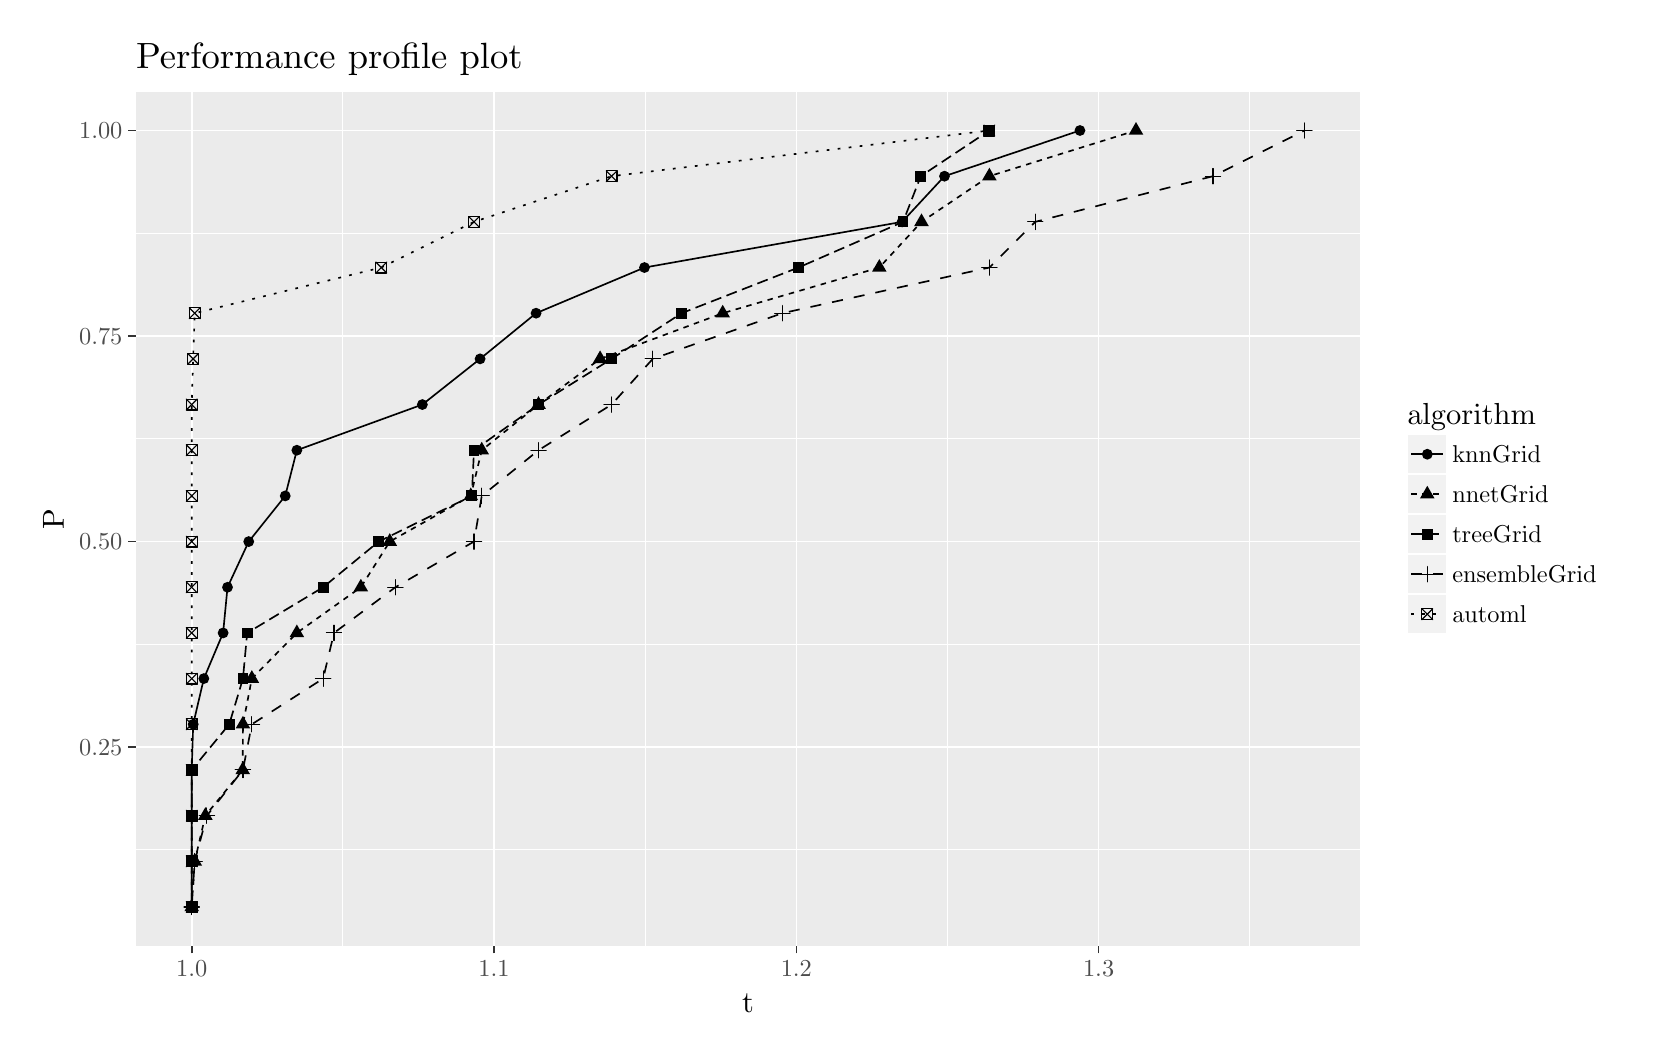
\begin{tikzpicture}[x=1pt,y=1pt]
\definecolor{fillColor}{RGB}{255,255,255}
\path[use as bounding box,fill=fillColor,fill opacity=0.00] (0,0) rectangle (578.16,361.35);
\begin{scope}
\path[clip] (  0.00,  0.00) rectangle (578.16,361.35);
\definecolor{drawColor}{RGB}{255,255,255}
\definecolor{fillColor}{RGB}{255,255,255}

\path[draw=drawColor,line width= 0.6pt,line join=round,line cap=round,fill=fillColor] (  0.00,  0.00) rectangle (578.16,361.35);
\end{scope}
\begin{scope}
\path[clip] ( 39.17, 29.59) rectangle (481.45,338.21);
\definecolor{fillColor}{gray}{0.92}

\path[fill=fillColor] ( 39.17, 29.59) rectangle (481.45,338.21);
\definecolor{drawColor}{RGB}{255,255,255}

\path[draw=drawColor,line width= 0.3pt,line join=round] ( 39.17, 64.25) --
	(481.45, 64.25);

\path[draw=drawColor,line width= 0.3pt,line join=round] ( 39.17,138.51) --
	(481.45,138.51);

\path[draw=drawColor,line width= 0.3pt,line join=round] ( 39.17,212.78) --
	(481.45,212.78);

\path[draw=drawColor,line width= 0.3pt,line join=round] ( 39.17,287.05) --
	(481.45,287.05);

\path[draw=drawColor,line width= 0.3pt,line join=round] (113.89, 29.59) --
	(113.89,338.21);

\path[draw=drawColor,line width= 0.3pt,line join=round] (223.13, 29.59) --
	(223.13,338.21);

\path[draw=drawColor,line width= 0.3pt,line join=round] (332.37, 29.59) --
	(332.37,338.21);

\path[draw=drawColor,line width= 0.3pt,line join=round] (441.61, 29.59) --
	(441.61,338.21);

\path[draw=drawColor,line width= 0.6pt,line join=round] ( 39.17,101.38) --
	(481.45,101.38);

\path[draw=drawColor,line width= 0.6pt,line join=round] ( 39.17,175.65) --
	(481.45,175.65);

\path[draw=drawColor,line width= 0.6pt,line join=round] ( 39.17,249.92) --
	(481.45,249.92);

\path[draw=drawColor,line width= 0.6pt,line join=round] ( 39.17,324.19) --
	(481.45,324.19);

\path[draw=drawColor,line width= 0.6pt,line join=round] ( 59.27, 29.59) --
	( 59.27,338.21);

\path[draw=drawColor,line width= 0.6pt,line join=round] (168.51, 29.59) --
	(168.51,338.21);

\path[draw=drawColor,line width= 0.6pt,line join=round] (277.75, 29.59) --
	(277.75,338.21);

\path[draw=drawColor,line width= 0.6pt,line join=round] (386.99, 29.59) --
	(386.99,338.21);
\definecolor{drawColor}{RGB}{0,0,0}

\path[draw=drawColor,line width= 0.6pt,line join=round] ( 59.27, 43.62) --
	( 59.27, 60.12) --
	( 59.27, 76.62) --
	( 59.27, 93.13) --
	( 59.81,109.63) --
	( 63.66,126.14) --
	( 70.62,142.64) --
	( 72.21,159.14) --
	( 79.88,175.65) --
	( 93.07,192.15) --
	( 97.27,208.66) --
	(142.62,225.16) --
	(163.48,241.67) --
	(183.71,258.17) --
	(222.88,274.67) --
	(315.97,291.18) --
	(331.29,307.68) --
	(380.23,324.19);

\path[draw=drawColor,line width= 0.6pt,dash pattern=on 2pt off 2pt ,line join=round] ( 59.27, 43.62) --
	( 60.36, 60.12) --
	( 64.21, 76.62) --
	( 77.71, 93.13) --
	( 77.79,109.63) --
	( 81.00,126.14) --
	( 97.27,142.64) --
	(120.40,159.14) --
	(130.84,175.65) --
	(160.12,192.15) --
	(164.08,208.66) --
	(184.60,225.16) --
	(206.85,241.67) --
	(251.15,258.17) --
	(307.74,274.67) --
	(322.98,291.18) --
	(347.51,307.68) --
	(400.49,324.19);

\path[draw=drawColor,line width= 0.6pt,dash pattern=on 4pt off 2pt ,line join=round] ( 59.27, 43.62) --
	( 59.27, 60.12) --
	( 59.27, 76.62) --
	( 59.27, 93.13) --
	( 72.83,109.63) --
	( 77.79,126.14) --
	( 79.32,142.64) --
	(106.77,159.14) --
	(126.84,175.65) --
	(160.49,192.15) --
	(161.28,208.66) --
	(184.60,225.16) --
	(211.00,241.67) --
	(236.29,258.17) --
	(278.51,274.67) --
	(316.32,291.18) --
	(322.71,307.68) --
	(347.51,324.19);

\path[draw=drawColor,line width= 0.6pt,dash pattern=on 4pt off 4pt ,line join=round] ( 59.27, 43.62) --
	( 60.36, 60.12) --
	( 64.76, 76.62) --
	( 77.79, 93.13) --
	( 81.00,109.63) --
	(106.77,126.14) --
	(110.69,142.64) --
	(132.86,159.14) --
	(161.28,175.65) --
	(164.08,192.15) --
	(184.60,208.66) --
	(211.00,225.16) --
	(225.88,241.67) --
	(272.69,258.17) --
	(347.51,274.67) --
	(364.08,291.18) --
	(428.32,307.68) --
	(461.34,324.19);

\path[draw=drawColor,line width= 0.6pt,dash pattern=on 1pt off 3pt ,line join=round] ( 59.27, 43.62) --
	( 59.27, 60.12) --
	( 59.27, 76.62) --
	( 59.27, 93.13) --
	( 59.27,109.63) --
	( 59.27,126.14) --
	( 59.27,142.64) --
	( 59.27,159.14) --
	( 59.27,175.65) --
	( 59.27,192.15) --
	( 59.27,208.66) --
	( 59.27,225.16) --
	( 59.79,241.67) --
	( 60.36,258.17) --
	(127.77,274.67) --
	(161.28,291.18) --
	(211.00,307.68) --
	(347.51,324.19);
\definecolor{fillColor}{RGB}{0,0,0}

\path[fill=fillColor] ( 59.27, 43.62) circle (  1.96);

\path[fill=fillColor] ( 59.27, 60.12) circle (  1.96);

\path[fill=fillColor] ( 59.27, 76.62) circle (  1.96);

\path[fill=fillColor] ( 59.27, 93.13) circle (  1.96);

\path[fill=fillColor] ( 59.81,109.63) circle (  1.96);

\path[fill=fillColor] ( 63.66,126.14) circle (  1.96);

\path[fill=fillColor] ( 70.62,142.64) circle (  1.96);

\path[fill=fillColor] ( 72.21,159.14) circle (  1.96);

\path[fill=fillColor] ( 79.88,175.65) circle (  1.96);

\path[fill=fillColor] ( 93.07,192.15) circle (  1.96);

\path[fill=fillColor] ( 97.27,208.66) circle (  1.96);

\path[fill=fillColor] (142.62,225.16) circle (  1.96);

\path[fill=fillColor] (163.48,241.67) circle (  1.96);

\path[fill=fillColor] (183.71,258.17) circle (  1.96);

\path[fill=fillColor] (222.88,274.67) circle (  1.96);

\path[fill=fillColor] (315.97,291.18) circle (  1.96);

\path[fill=fillColor] (331.29,307.68) circle (  1.96);

\path[fill=fillColor] (380.23,324.19) circle (  1.96);

\path[fill=fillColor] ( 59.27, 46.67) --
	( 61.91, 42.09) --
	( 56.63, 42.09) --
	cycle;

\path[fill=fillColor] ( 60.36, 63.17) --
	( 63.00, 58.59) --
	( 57.72, 58.59) --
	cycle;

\path[fill=fillColor] ( 64.21, 79.67) --
	( 66.85, 75.10) --
	( 61.57, 75.10) --
	cycle;

\path[fill=fillColor] ( 77.71, 96.18) --
	( 80.35, 91.60) --
	( 75.07, 91.60) --
	cycle;

\path[fill=fillColor] ( 77.79,112.68) --
	( 80.43,108.11) --
	( 75.14,108.11) --
	cycle;

\path[fill=fillColor] ( 81.00,129.19) --
	( 83.64,124.61) --
	( 78.35,124.61) --
	cycle;

\path[fill=fillColor] ( 97.27,145.69) --
	( 99.91,141.11) --
	( 94.62,141.11) --
	cycle;

\path[fill=fillColor] (120.40,162.20) --
	(123.04,157.62) --
	(117.75,157.62) --
	cycle;

\path[fill=fillColor] (130.84,178.70) --
	(133.49,174.12) --
	(128.20,174.12) --
	cycle;

\path[fill=fillColor] (160.12,195.20) --
	(162.76,190.63) --
	(157.48,190.63) --
	cycle;

\path[fill=fillColor] (164.08,211.71) --
	(166.72,207.13) --
	(161.44,207.13) --
	cycle;

\path[fill=fillColor] (184.60,228.21) --
	(187.24,223.64) --
	(181.96,223.64) --
	cycle;

\path[fill=fillColor] (206.85,244.72) --
	(209.49,240.14) --
	(204.21,240.14) --
	cycle;

\path[fill=fillColor] (251.15,261.22) --
	(253.79,256.64) --
	(248.51,256.64) --
	cycle;

\path[fill=fillColor] (307.74,277.73) --
	(310.38,273.15) --
	(305.10,273.15) --
	cycle;

\path[fill=fillColor] (322.98,294.23) --
	(325.62,289.65) --
	(320.33,289.65) --
	cycle;

\path[fill=fillColor] (347.51,310.73) --
	(350.15,306.16) --
	(344.86,306.16) --
	cycle;

\path[fill=fillColor] (400.49,327.24) --
	(403.14,322.66) --
	(397.85,322.66) --
	cycle;

\path[fill=fillColor] ( 57.31, 41.65) --
	( 61.23, 41.65) --
	( 61.23, 45.58) --
	( 57.31, 45.58) --
	cycle;

\path[fill=fillColor] ( 57.31, 58.16) --
	( 61.23, 58.16) --
	( 61.23, 62.08) --
	( 57.31, 62.08) --
	cycle;

\path[fill=fillColor] ( 57.31, 74.66) --
	( 61.23, 74.66) --
	( 61.23, 78.59) --
	( 57.31, 78.59) --
	cycle;

\path[fill=fillColor] ( 57.31, 91.17) --
	( 61.23, 91.17) --
	( 61.23, 95.09) --
	( 57.31, 95.09) --
	cycle;

\path[fill=fillColor] ( 70.87,107.67) --
	( 74.79,107.67) --
	( 74.79,111.59) --
	( 70.87,111.59) --
	cycle;

\path[fill=fillColor] ( 75.82,124.17) --
	( 79.75,124.17) --
	( 79.75,128.10) --
	( 75.82,128.10) --
	cycle;

\path[fill=fillColor] ( 77.36,140.68) --
	( 81.29,140.68) --
	( 81.29,144.60) --
	( 77.36,144.60) --
	cycle;

\path[fill=fillColor] (104.80,157.18) --
	(108.73,157.18) --
	(108.73,161.11) --
	(104.80,161.11) --
	cycle;

\path[fill=fillColor] (124.87,173.69) --
	(128.80,173.69) --
	(128.80,177.61) --
	(124.87,177.61) --
	cycle;

\path[fill=fillColor] (158.53,190.19) --
	(162.45,190.19) --
	(162.45,194.12) --
	(158.53,194.12) --
	cycle;

\path[fill=fillColor] (159.32,206.69) --
	(163.24,206.69) --
	(163.24,210.62) --
	(159.32,210.62) --
	cycle;

\path[fill=fillColor] (182.64,223.20) --
	(186.56,223.20) --
	(186.56,227.12) --
	(182.64,227.12) --
	cycle;

\path[fill=fillColor] (209.03,239.70) --
	(212.96,239.70) --
	(212.96,243.63) --
	(209.03,243.63) --
	cycle;

\path[fill=fillColor] (234.33,256.21) --
	(238.25,256.21) --
	(238.25,260.13) --
	(234.33,260.13) --
	cycle;

\path[fill=fillColor] (276.54,272.71) --
	(280.47,272.71) --
	(280.47,276.64) --
	(276.54,276.64) --
	cycle;

\path[fill=fillColor] (314.36,289.22) --
	(318.28,289.22) --
	(318.28,293.14) --
	(314.36,293.14) --
	cycle;

\path[fill=fillColor] (320.75,305.72) --
	(324.67,305.72) --
	(324.67,309.64) --
	(320.75,309.64) --
	cycle;

\path[fill=fillColor] (345.54,322.22) --
	(349.47,322.22) --
	(349.47,326.15) --
	(345.54,326.15) --
	cycle;

\path[draw=drawColor,line width= 0.4pt,line join=round,line cap=round] ( 56.50, 43.62) -- ( 62.05, 43.62);

\path[draw=drawColor,line width= 0.4pt,line join=round,line cap=round] ( 59.27, 40.84) -- ( 59.27, 46.39);

\path[draw=drawColor,line width= 0.4pt,line join=round,line cap=round] ( 57.59, 60.12) -- ( 63.14, 60.12);

\path[draw=drawColor,line width= 0.4pt,line join=round,line cap=round] ( 60.36, 57.34) -- ( 60.36, 62.89);

\path[draw=drawColor,line width= 0.4pt,line join=round,line cap=round] ( 61.98, 76.62) -- ( 67.53, 76.62);

\path[draw=drawColor,line width= 0.4pt,line join=round,line cap=round] ( 64.76, 73.85) -- ( 64.76, 79.40);

\path[draw=drawColor,line width= 0.4pt,line join=round,line cap=round] ( 75.01, 93.13) -- ( 80.56, 93.13);

\path[draw=drawColor,line width= 0.4pt,line join=round,line cap=round] ( 77.79, 90.35) -- ( 77.79, 95.90);

\path[draw=drawColor,line width= 0.4pt,line join=round,line cap=round] ( 78.22,109.63) -- ( 83.77,109.63);

\path[draw=drawColor,line width= 0.4pt,line join=round,line cap=round] ( 81.00,106.86) -- ( 81.00,112.41);

\path[draw=drawColor,line width= 0.4pt,line join=round,line cap=round] (103.99,126.14) -- (109.54,126.14);

\path[draw=drawColor,line width= 0.4pt,line join=round,line cap=round] (106.77,123.36) -- (106.77,128.91);

\path[draw=drawColor,line width= 0.4pt,line join=round,line cap=round] (107.91,142.64) -- (113.46,142.64);

\path[draw=drawColor,line width= 0.4pt,line join=round,line cap=round] (110.69,139.87) -- (110.69,145.42);

\path[draw=drawColor,line width= 0.4pt,line join=round,line cap=round] (130.09,159.14) -- (135.64,159.14);

\path[draw=drawColor,line width= 0.4pt,line join=round,line cap=round] (132.86,156.37) -- (132.86,161.92);

\path[draw=drawColor,line width= 0.4pt,line join=round,line cap=round] (158.51,175.65) -- (164.06,175.65);

\path[draw=drawColor,line width= 0.4pt,line join=round,line cap=round] (161.28,172.87) -- (161.28,178.42);

\path[draw=drawColor,line width= 0.4pt,line join=round,line cap=round] (161.30,192.15) -- (166.85,192.15);

\path[draw=drawColor,line width= 0.4pt,line join=round,line cap=round] (164.08,189.38) -- (164.08,194.93);

\path[draw=drawColor,line width= 0.4pt,line join=round,line cap=round] (181.82,208.66) -- (187.37,208.66);

\path[draw=drawColor,line width= 0.4pt,line join=round,line cap=round] (184.60,205.88) -- (184.60,211.43);

\path[draw=drawColor,line width= 0.4pt,line join=round,line cap=round] (208.22,225.16) -- (213.77,225.16);

\path[draw=drawColor,line width= 0.4pt,line join=round,line cap=round] (211.00,222.39) -- (211.00,227.94);

\path[draw=drawColor,line width= 0.4pt,line join=round,line cap=round] (223.11,241.67) -- (228.66,241.67);

\path[draw=drawColor,line width= 0.4pt,line join=round,line cap=round] (225.88,238.89) -- (225.88,244.44);

\path[draw=drawColor,line width= 0.4pt,line join=round,line cap=round] (269.92,258.17) -- (275.47,258.17);

\path[draw=drawColor,line width= 0.4pt,line join=round,line cap=round] (272.69,255.39) -- (272.69,260.94);

\path[draw=drawColor,line width= 0.4pt,line join=round,line cap=round] (344.73,274.67) -- (350.28,274.67);

\path[draw=drawColor,line width= 0.4pt,line join=round,line cap=round] (347.51,271.90) -- (347.51,277.45);

\path[draw=drawColor,line width= 0.4pt,line join=round,line cap=round] (361.31,291.18) -- (366.86,291.18);

\path[draw=drawColor,line width= 0.4pt,line join=round,line cap=round] (364.08,288.40) -- (364.08,293.95);

\path[draw=drawColor,line width= 0.4pt,line join=round,line cap=round] (425.55,307.68) -- (431.09,307.68);

\path[draw=drawColor,line width= 0.4pt,line join=round,line cap=round] (428.32,304.91) -- (428.32,310.46);

\path[draw=drawColor,line width= 0.4pt,line join=round,line cap=round] (458.57,324.19) -- (464.12,324.19);

\path[draw=drawColor,line width= 0.4pt,line join=round,line cap=round] (461.34,321.41) -- (461.34,326.96);

\path[draw=drawColor,line width= 0.4pt,line join=round,line cap=round] ( 57.31, 41.65) rectangle ( 61.23, 45.58);

\path[draw=drawColor,line width= 0.4pt,line join=round,line cap=round] ( 57.31, 41.65) -- ( 61.23, 45.58);

\path[draw=drawColor,line width= 0.4pt,line join=round,line cap=round] ( 57.31, 45.58) -- ( 61.23, 41.65);

\path[draw=drawColor,line width= 0.4pt,line join=round,line cap=round] ( 57.31, 58.16) rectangle ( 61.23, 62.08);

\path[draw=drawColor,line width= 0.4pt,line join=round,line cap=round] ( 57.31, 58.16) -- ( 61.23, 62.08);

\path[draw=drawColor,line width= 0.4pt,line join=round,line cap=round] ( 57.31, 62.08) -- ( 61.23, 58.16);

\path[draw=drawColor,line width= 0.4pt,line join=round,line cap=round] ( 57.31, 74.66) rectangle ( 61.23, 78.59);

\path[draw=drawColor,line width= 0.4pt,line join=round,line cap=round] ( 57.31, 74.66) -- ( 61.23, 78.59);

\path[draw=drawColor,line width= 0.4pt,line join=round,line cap=round] ( 57.31, 78.59) -- ( 61.23, 74.66);

\path[draw=drawColor,line width= 0.4pt,line join=round,line cap=round] ( 57.31, 91.17) rectangle ( 61.23, 95.09);

\path[draw=drawColor,line width= 0.4pt,line join=round,line cap=round] ( 57.31, 91.17) -- ( 61.23, 95.09);

\path[draw=drawColor,line width= 0.4pt,line join=round,line cap=round] ( 57.31, 95.09) -- ( 61.23, 91.17);

\path[draw=drawColor,line width= 0.4pt,line join=round,line cap=round] ( 57.31,107.67) rectangle ( 61.23,111.59);

\path[draw=drawColor,line width= 0.4pt,line join=round,line cap=round] ( 57.31,107.67) -- ( 61.23,111.59);

\path[draw=drawColor,line width= 0.4pt,line join=round,line cap=round] ( 57.31,111.59) -- ( 61.23,107.67);

\path[draw=drawColor,line width= 0.4pt,line join=round,line cap=round] ( 57.31,124.17) rectangle ( 61.23,128.10);

\path[draw=drawColor,line width= 0.4pt,line join=round,line cap=round] ( 57.31,124.17) -- ( 61.23,128.10);

\path[draw=drawColor,line width= 0.4pt,line join=round,line cap=round] ( 57.31,128.10) -- ( 61.23,124.17);

\path[draw=drawColor,line width= 0.4pt,line join=round,line cap=round] ( 57.31,140.68) rectangle ( 61.23,144.60);

\path[draw=drawColor,line width= 0.4pt,line join=round,line cap=round] ( 57.31,140.68) -- ( 61.23,144.60);

\path[draw=drawColor,line width= 0.4pt,line join=round,line cap=round] ( 57.31,144.60) -- ( 61.23,140.68);

\path[draw=drawColor,line width= 0.4pt,line join=round,line cap=round] ( 57.31,157.18) rectangle ( 61.23,161.11);

\path[draw=drawColor,line width= 0.4pt,line join=round,line cap=round] ( 57.31,157.18) -- ( 61.23,161.11);

\path[draw=drawColor,line width= 0.4pt,line join=round,line cap=round] ( 57.31,161.11) -- ( 61.23,157.18);

\path[draw=drawColor,line width= 0.4pt,line join=round,line cap=round] ( 57.31,173.69) rectangle ( 61.23,177.61);

\path[draw=drawColor,line width= 0.4pt,line join=round,line cap=round] ( 57.31,173.69) -- ( 61.23,177.61);

\path[draw=drawColor,line width= 0.4pt,line join=round,line cap=round] ( 57.31,177.61) -- ( 61.23,173.69);

\path[draw=drawColor,line width= 0.4pt,line join=round,line cap=round] ( 57.31,190.19) rectangle ( 61.23,194.12);

\path[draw=drawColor,line width= 0.4pt,line join=round,line cap=round] ( 57.31,190.19) -- ( 61.23,194.12);

\path[draw=drawColor,line width= 0.4pt,line join=round,line cap=round] ( 57.31,194.12) -- ( 61.23,190.19);

\path[draw=drawColor,line width= 0.4pt,line join=round,line cap=round] ( 57.31,206.69) rectangle ( 61.23,210.62);

\path[draw=drawColor,line width= 0.4pt,line join=round,line cap=round] ( 57.31,206.69) -- ( 61.23,210.62);

\path[draw=drawColor,line width= 0.4pt,line join=round,line cap=round] ( 57.31,210.62) -- ( 61.23,206.69);

\path[draw=drawColor,line width= 0.4pt,line join=round,line cap=round] ( 57.31,223.20) rectangle ( 61.23,227.12);

\path[draw=drawColor,line width= 0.4pt,line join=round,line cap=round] ( 57.31,223.20) -- ( 61.23,227.12);

\path[draw=drawColor,line width= 0.4pt,line join=round,line cap=round] ( 57.31,227.12) -- ( 61.23,223.20);

\path[draw=drawColor,line width= 0.4pt,line join=round,line cap=round] ( 57.83,239.70) rectangle ( 61.75,243.63);

\path[draw=drawColor,line width= 0.4pt,line join=round,line cap=round] ( 57.83,239.70) -- ( 61.75,243.63);

\path[draw=drawColor,line width= 0.4pt,line join=round,line cap=round] ( 57.83,243.63) -- ( 61.75,239.70);

\path[draw=drawColor,line width= 0.4pt,line join=round,line cap=round] ( 58.40,256.21) rectangle ( 62.32,260.13);

\path[draw=drawColor,line width= 0.4pt,line join=round,line cap=round] ( 58.40,256.21) -- ( 62.32,260.13);

\path[draw=drawColor,line width= 0.4pt,line join=round,line cap=round] ( 58.40,260.13) -- ( 62.32,256.21);

\path[draw=drawColor,line width= 0.4pt,line join=round,line cap=round] (125.81,272.71) rectangle (129.73,276.64);

\path[draw=drawColor,line width= 0.4pt,line join=round,line cap=round] (125.81,272.71) -- (129.73,276.64);

\path[draw=drawColor,line width= 0.4pt,line join=round,line cap=round] (125.81,276.64) -- (129.73,272.71);

\path[draw=drawColor,line width= 0.4pt,line join=round,line cap=round] (159.32,289.22) rectangle (163.24,293.14);

\path[draw=drawColor,line width= 0.4pt,line join=round,line cap=round] (159.32,289.22) -- (163.24,293.14);

\path[draw=drawColor,line width= 0.4pt,line join=round,line cap=round] (159.32,293.14) -- (163.24,289.22);

\path[draw=drawColor,line width= 0.4pt,line join=round,line cap=round] (209.03,305.72) rectangle (212.96,309.64);

\path[draw=drawColor,line width= 0.4pt,line join=round,line cap=round] (209.03,305.72) -- (212.96,309.64);

\path[draw=drawColor,line width= 0.4pt,line join=round,line cap=round] (209.03,309.64) -- (212.96,305.72);

\path[draw=drawColor,line width= 0.4pt,line join=round,line cap=round] (345.54,322.22) rectangle (349.47,326.15);

\path[draw=drawColor,line width= 0.4pt,line join=round,line cap=round] (345.54,322.22) -- (349.47,326.15);

\path[draw=drawColor,line width= 0.4pt,line join=round,line cap=round] (345.54,326.15) -- (349.47,322.22);
\end{scope}
\begin{scope}
\path[clip] (  0.00,  0.00) rectangle (578.16,361.35);
\definecolor{drawColor}{gray}{0.30}

\node[text=drawColor,anchor=base east,inner sep=0pt, outer sep=0pt, scale=  0.88] at ( 34.22, 98.35) {0.25};

\node[text=drawColor,anchor=base east,inner sep=0pt, outer sep=0pt, scale=  0.88] at ( 34.22,172.62) {0.50};

\node[text=drawColor,anchor=base east,inner sep=0pt, outer sep=0pt, scale=  0.88] at ( 34.22,246.89) {0.75};

\node[text=drawColor,anchor=base east,inner sep=0pt, outer sep=0pt, scale=  0.88] at ( 34.22,321.16) {1.00};
\end{scope}
\begin{scope}
\path[clip] (  0.00,  0.00) rectangle (578.16,361.35);
\definecolor{drawColor}{gray}{0.20}

\path[draw=drawColor,line width= 0.6pt,line join=round] ( 36.42,101.38) --
	( 39.17,101.38);

\path[draw=drawColor,line width= 0.6pt,line join=round] ( 36.42,175.65) --
	( 39.17,175.65);

\path[draw=drawColor,line width= 0.6pt,line join=round] ( 36.42,249.92) --
	( 39.17,249.92);

\path[draw=drawColor,line width= 0.6pt,line join=round] ( 36.42,324.19) --
	( 39.17,324.19);
\end{scope}
\begin{scope}
\path[clip] (  0.00,  0.00) rectangle (578.16,361.35);
\definecolor{drawColor}{gray}{0.20}

\path[draw=drawColor,line width= 0.6pt,line join=round] ( 59.27, 26.84) --
	( 59.27, 29.59);

\path[draw=drawColor,line width= 0.6pt,line join=round] (168.51, 26.84) --
	(168.51, 29.59);

\path[draw=drawColor,line width= 0.6pt,line join=round] (277.75, 26.84) --
	(277.75, 29.59);

\path[draw=drawColor,line width= 0.6pt,line join=round] (386.99, 26.84) --
	(386.99, 29.59);
\end{scope}
\begin{scope}
\path[clip] (  0.00,  0.00) rectangle (578.16,361.35);
\definecolor{drawColor}{gray}{0.30}

\node[text=drawColor,anchor=base,inner sep=0pt, outer sep=0pt, scale=  0.88] at ( 59.27, 18.58) {1.0};

\node[text=drawColor,anchor=base,inner sep=0pt, outer sep=0pt, scale=  0.88] at (168.51, 18.58) {1.1};

\node[text=drawColor,anchor=base,inner sep=0pt, outer sep=0pt, scale=  0.88] at (277.75, 18.58) {1.2};

\node[text=drawColor,anchor=base,inner sep=0pt, outer sep=0pt, scale=  0.88] at (386.99, 18.58) {1.3};
\end{scope}
\begin{scope}
\path[clip] (  0.00,  0.00) rectangle (578.16,361.35);
\definecolor{drawColor}{RGB}{0,0,0}

\node[text=drawColor,anchor=base,inner sep=0pt, outer sep=0pt, scale=  1.10] at (260.31,  5.50) {t};
\end{scope}
\begin{scope}
\path[clip] (  0.00,  0.00) rectangle (578.16,361.35);
\definecolor{drawColor}{RGB}{0,0,0}

\node[text=drawColor,rotate= 90.00,anchor=base,inner sep=0pt, outer sep=0pt, scale=  1.10] at ( 13.08,183.90) {P};
\end{scope}
\begin{scope}
\path[clip] (  0.00,  0.00) rectangle (578.16,361.35);
\definecolor{fillColor}{RGB}{255,255,255}

\path[fill=fillColor] (492.83,136.48) rectangle (572.66,231.32);
\end{scope}
\begin{scope}
\path[clip] (  0.00,  0.00) rectangle (578.16,361.35);
\definecolor{drawColor}{RGB}{0,0,0}

\node[text=drawColor,anchor=base west,inner sep=0pt, outer sep=0pt, scale=  1.10] at (498.52,218.05) {algorithm};
\end{scope}
\begin{scope}
\path[clip] (  0.00,  0.00) rectangle (578.16,361.35);
\definecolor{drawColor}{RGB}{255,255,255}
\definecolor{fillColor}{gray}{0.95}

\path[draw=drawColor,line width= 0.6pt,line join=round,line cap=round,fill=fillColor] (498.52,199.99) rectangle (512.97,214.44);
\end{scope}
\begin{scope}
\path[clip] (  0.00,  0.00) rectangle (578.16,361.35);
\definecolor{drawColor}{RGB}{0,0,0}

\path[draw=drawColor,line width= 0.6pt,line join=round] (499.97,207.21) -- (511.53,207.21);
\end{scope}
\begin{scope}
\path[clip] (  0.00,  0.00) rectangle (578.16,361.35);
\definecolor{fillColor}{RGB}{0,0,0}

\path[fill=fillColor] (505.75,207.21) circle (  1.96);
\end{scope}
\begin{scope}
\path[clip] (  0.00,  0.00) rectangle (578.16,361.35);
\definecolor{drawColor}{RGB}{255,255,255}
\definecolor{fillColor}{gray}{0.95}

\path[draw=drawColor,line width= 0.6pt,line join=round,line cap=round,fill=fillColor] (498.52,185.53) rectangle (512.97,199.99);
\end{scope}
\begin{scope}
\path[clip] (  0.00,  0.00) rectangle (578.16,361.35);
\definecolor{drawColor}{RGB}{0,0,0}

\path[draw=drawColor,line width= 0.6pt,dash pattern=on 2pt off 2pt ,line join=round] (499.97,192.76) -- (511.53,192.76);
\end{scope}
\begin{scope}
\path[clip] (  0.00,  0.00) rectangle (578.16,361.35);
\definecolor{fillColor}{RGB}{0,0,0}

\path[fill=fillColor] (505.75,195.81) --
	(508.39,191.23) --
	(503.10,191.23) --
	cycle;
\end{scope}
\begin{scope}
\path[clip] (  0.00,  0.00) rectangle (578.16,361.35);
\definecolor{drawColor}{RGB}{255,255,255}
\definecolor{fillColor}{gray}{0.95}

\path[draw=drawColor,line width= 0.6pt,line join=round,line cap=round,fill=fillColor] (498.52,171.08) rectangle (512.97,185.53);
\end{scope}
\begin{scope}
\path[clip] (  0.00,  0.00) rectangle (578.16,361.35);
\definecolor{drawColor}{RGB}{0,0,0}

\path[draw=drawColor,line width= 0.6pt,dash pattern=on 4pt off 2pt ,line join=round] (499.97,178.31) -- (511.53,178.31);
\end{scope}
\begin{scope}
\path[clip] (  0.00,  0.00) rectangle (578.16,361.35);
\definecolor{fillColor}{RGB}{0,0,0}

\path[fill=fillColor] (503.78,176.34) --
	(507.71,176.34) --
	(507.71,180.27) --
	(503.78,180.27) --
	cycle;
\end{scope}
\begin{scope}
\path[clip] (  0.00,  0.00) rectangle (578.16,361.35);
\definecolor{drawColor}{RGB}{255,255,255}
\definecolor{fillColor}{gray}{0.95}

\path[draw=drawColor,line width= 0.6pt,line join=round,line cap=round,fill=fillColor] (498.52,156.63) rectangle (512.97,171.08);
\end{scope}
\begin{scope}
\path[clip] (  0.00,  0.00) rectangle (578.16,361.35);
\definecolor{drawColor}{RGB}{0,0,0}

\path[draw=drawColor,line width= 0.6pt,dash pattern=on 4pt off 4pt ,line join=round] (499.97,163.85) -- (511.53,163.85);
\end{scope}
\begin{scope}
\path[clip] (  0.00,  0.00) rectangle (578.16,361.35);
\definecolor{drawColor}{RGB}{0,0,0}

\path[draw=drawColor,line width= 0.4pt,line join=round,line cap=round] (502.97,163.85) -- (508.52,163.85);

\path[draw=drawColor,line width= 0.4pt,line join=round,line cap=round] (505.75,161.08) -- (505.75,166.63);
\end{scope}
\begin{scope}
\path[clip] (  0.00,  0.00) rectangle (578.16,361.35);
\definecolor{drawColor}{RGB}{255,255,255}
\definecolor{fillColor}{gray}{0.95}

\path[draw=drawColor,line width= 0.6pt,line join=round,line cap=round,fill=fillColor] (498.52,142.17) rectangle (512.97,156.63);
\end{scope}
\begin{scope}
\path[clip] (  0.00,  0.00) rectangle (578.16,361.35);
\definecolor{drawColor}{RGB}{0,0,0}

\path[draw=drawColor,line width= 0.6pt,dash pattern=on 1pt off 3pt ,line join=round] (499.97,149.40) -- (511.53,149.40);
\end{scope}
\begin{scope}
\path[clip] (  0.00,  0.00) rectangle (578.16,361.35);
\definecolor{drawColor}{RGB}{0,0,0}

\path[draw=drawColor,line width= 0.4pt,line join=round,line cap=round] (503.78,147.44) rectangle (507.71,151.36);

\path[draw=drawColor,line width= 0.4pt,line join=round,line cap=round] (503.78,147.44) -- (507.71,151.36);

\path[draw=drawColor,line width= 0.4pt,line join=round,line cap=round] (503.78,151.36) -- (507.71,147.44);
\end{scope}
\begin{scope}
\path[clip] (  0.00,  0.00) rectangle (578.16,361.35);
\definecolor{drawColor}{RGB}{0,0,0}

\node[text=drawColor,anchor=base west,inner sep=0pt, outer sep=0pt, scale=  0.88] at (514.78,204.18) {knnGrid};
\end{scope}
\begin{scope}
\path[clip] (  0.00,  0.00) rectangle (578.16,361.35);
\definecolor{drawColor}{RGB}{0,0,0}

\node[text=drawColor,anchor=base west,inner sep=0pt, outer sep=0pt, scale=  0.88] at (514.78,189.73) {nnetGrid};
\end{scope}
\begin{scope}
\path[clip] (  0.00,  0.00) rectangle (578.16,361.35);
\definecolor{drawColor}{RGB}{0,0,0}

\node[text=drawColor,anchor=base west,inner sep=0pt, outer sep=0pt, scale=  0.88] at (514.78,175.28) {treeGrid};
\end{scope}
\begin{scope}
\path[clip] (  0.00,  0.00) rectangle (578.16,361.35);
\definecolor{drawColor}{RGB}{0,0,0}

\node[text=drawColor,anchor=base west,inner sep=0pt, outer sep=0pt, scale=  0.88] at (514.78,160.82) {ensembleGrid};
\end{scope}
\begin{scope}
\path[clip] (  0.00,  0.00) rectangle (578.16,361.35);
\definecolor{drawColor}{RGB}{0,0,0}

\node[text=drawColor,anchor=base west,inner sep=0pt, outer sep=0pt, scale=  0.88] at (514.78,146.37) {automl};
\end{scope}
\begin{scope}
\path[clip] (  0.00,  0.00) rectangle (578.16,361.35);
\definecolor{drawColor}{RGB}{0,0,0}

\node[text=drawColor,anchor=base west,inner sep=0pt, outer sep=0pt, scale=  1.32] at ( 39.17,346.76) {Performance profile plot};
\end{scope}
\end{tikzpicture}

}
  	\end{figure}
  \end{frame}
    \begin{frame}{Αξιολόγηση συστήματος: σύγκριση με Bayesian βελτιστοποίηση} 
    	\begin{figure}[!htb]
    		\scalebox{0.5}{
    			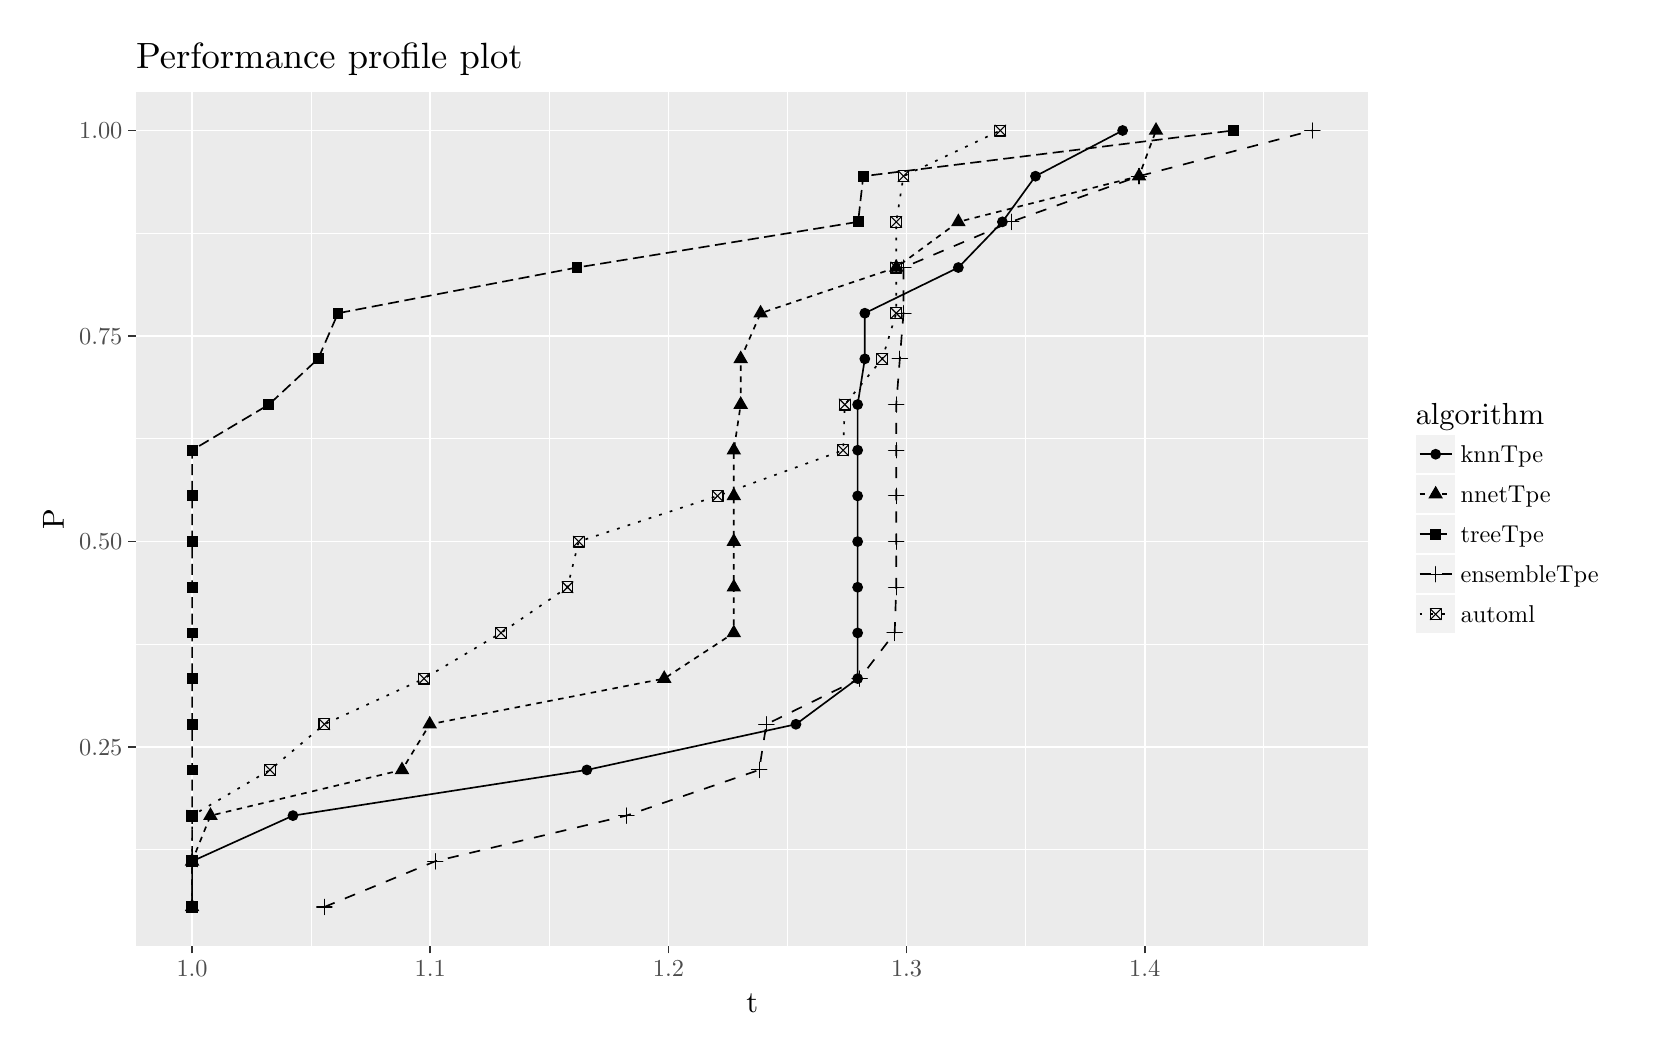
\begin{tikzpicture}[x=1pt,y=1pt]
\definecolor{fillColor}{RGB}{255,255,255}
\path[use as bounding box,fill=fillColor,fill opacity=0.00] (0,0) rectangle (578.16,361.35);
\begin{scope}
\path[clip] (  0.00,  0.00) rectangle (578.16,361.35);
\definecolor{drawColor}{RGB}{255,255,255}
\definecolor{fillColor}{RGB}{255,255,255}

\path[draw=drawColor,line width= 0.6pt,line join=round,line cap=round,fill=fillColor] (  0.00,  0.00) rectangle (578.16,361.35);
\end{scope}
\begin{scope}
\path[clip] ( 39.17, 29.59) rectangle (484.47,338.21);
\definecolor{fillColor}{gray}{0.92}

\path[fill=fillColor] ( 39.17, 29.59) rectangle (484.47,338.21);
\definecolor{drawColor}{RGB}{255,255,255}

\path[draw=drawColor,line width= 0.3pt,line join=round] ( 39.17, 64.25) --
	(484.47, 64.25);

\path[draw=drawColor,line width= 0.3pt,line join=round] ( 39.17,138.51) --
	(484.47,138.51);

\path[draw=drawColor,line width= 0.3pt,line join=round] ( 39.17,212.78) --
	(484.47,212.78);

\path[draw=drawColor,line width= 0.3pt,line join=round] ( 39.17,287.05) --
	(484.47,287.05);

\path[draw=drawColor,line width= 0.3pt,line join=round] (102.44, 29.59) --
	(102.44,338.21);

\path[draw=drawColor,line width= 0.3pt,line join=round] (188.50, 29.59) --
	(188.50,338.21);

\path[draw=drawColor,line width= 0.3pt,line join=round] (274.56, 29.59) --
	(274.56,338.21);

\path[draw=drawColor,line width= 0.3pt,line join=round] (360.62, 29.59) --
	(360.62,338.21);

\path[draw=drawColor,line width= 0.3pt,line join=round] (446.68, 29.59) --
	(446.68,338.21);

\path[draw=drawColor,line width= 0.6pt,line join=round] ( 39.17,101.38) --
	(484.47,101.38);

\path[draw=drawColor,line width= 0.6pt,line join=round] ( 39.17,175.65) --
	(484.47,175.65);

\path[draw=drawColor,line width= 0.6pt,line join=round] ( 39.17,249.92) --
	(484.47,249.92);

\path[draw=drawColor,line width= 0.6pt,line join=round] ( 39.17,324.19) --
	(484.47,324.19);

\path[draw=drawColor,line width= 0.6pt,line join=round] ( 59.41, 29.59) --
	( 59.41,338.21);

\path[draw=drawColor,line width= 0.6pt,line join=round] (145.47, 29.59) --
	(145.47,338.21);

\path[draw=drawColor,line width= 0.6pt,line join=round] (231.53, 29.59) --
	(231.53,338.21);

\path[draw=drawColor,line width= 0.6pt,line join=round] (317.59, 29.59) --
	(317.59,338.21);

\path[draw=drawColor,line width= 0.6pt,line join=round] (403.65, 29.59) --
	(403.65,338.21);
\definecolor{drawColor}{RGB}{0,0,0}

\path[draw=drawColor,line width= 0.6pt,line join=round] ( 59.41, 43.62) --
	( 59.41, 60.12) --
	( 95.86, 76.62) --
	(202.06, 93.13) --
	(277.61,109.63) --
	(299.91,126.14) --
	(299.91,142.64) --
	(299.91,159.14) --
	(299.91,175.65) --
	(299.91,192.15) --
	(299.91,208.66) --
	(299.91,225.16) --
	(302.50,241.67) --
	(302.50,258.17) --
	(336.30,274.67) --
	(352.21,291.18) --
	(364.17,307.68) --
	(395.66,324.19);

\path[draw=drawColor,line width= 0.6pt,dash pattern=on 2pt off 2pt ,line join=round] ( 59.41, 43.62) --
	( 59.41, 60.12) --
	( 66.06, 76.62) --
	(135.27, 93.13) --
	(145.28,109.63) --
	(230.01,126.14) --
	(255.16,142.64) --
	(255.16,159.14) --
	(255.16,175.65) --
	(255.16,192.15) --
	(255.16,208.66) --
	(257.65,225.16) --
	(257.65,241.67) --
	(264.84,258.17) --
	(313.85,274.67) --
	(336.30,291.18) --
	(401.58,307.68) --
	(407.72,324.19);

\path[draw=drawColor,line width= 0.6pt,dash pattern=on 4pt off 2pt ,line join=round] ( 59.41, 43.62) --
	( 59.41, 60.12) --
	( 59.41, 76.62) --
	( 59.41, 93.13) --
	( 59.41,109.63) --
	( 59.41,126.14) --
	( 59.41,142.64) --
	( 59.41,159.14) --
	( 59.41,175.65) --
	( 59.41,192.15) --
	( 59.41,208.66) --
	( 87.17,225.16) --
	(104.94,241.67) --
	(112.15,258.17) --
	(198.50,274.67) --
	(300.08,291.18) --
	(301.93,307.68) --
	(435.58,324.19);

\path[draw=drawColor,line width= 0.6pt,dash pattern=on 4pt off 4pt ,line join=round] (107.22, 43.62) --
	(147.27, 60.12) --
	(216.33, 76.62) --
	(264.31, 93.13) --
	(266.93,109.63) --
	(300.64,126.14) --
	(313.29,142.64) --
	(313.85,159.14) --
	(313.85,175.65) --
	(313.85,192.15) --
	(313.85,208.66) --
	(313.85,225.16) --
	(315.15,241.67) --
	(316.47,258.17) --
	(316.47,274.67) --
	(355.35,291.18) --
	(401.58,307.68) --
	(464.23,324.19);

\path[draw=drawColor,line width= 0.6pt,dash pattern=on 1pt off 3pt ,line join=round] ( 59.41, 43.62) --
	( 59.41, 60.12) --
	( 59.41, 76.62) --
	( 87.56, 93.13) --
	(107.22,109.63) --
	(143.22,126.14) --
	(171.03,142.64) --
	(195.06,159.14) --
	(199.09,175.65) --
	(249.29,192.15) --
	(294.68,208.66) --
	(295.26,225.16) --
	(308.80,241.67) --
	(313.85,258.17) --
	(313.85,274.67) --
	(313.85,291.18) --
	(316.47,307.68) --
	(351.46,324.19);
\definecolor{fillColor}{RGB}{0,0,0}

\path[fill=fillColor] ( 59.41, 43.62) circle (  1.96);

\path[fill=fillColor] ( 59.41, 60.12) circle (  1.96);

\path[fill=fillColor] ( 95.86, 76.62) circle (  1.96);

\path[fill=fillColor] (202.06, 93.13) circle (  1.96);

\path[fill=fillColor] (277.61,109.63) circle (  1.96);

\path[fill=fillColor] (299.91,126.14) circle (  1.96);

\path[fill=fillColor] (299.91,142.64) circle (  1.96);

\path[fill=fillColor] (299.91,159.14) circle (  1.96);

\path[fill=fillColor] (299.91,175.65) circle (  1.96);

\path[fill=fillColor] (299.91,192.15) circle (  1.96);

\path[fill=fillColor] (299.91,208.66) circle (  1.96);

\path[fill=fillColor] (299.91,225.16) circle (  1.96);

\path[fill=fillColor] (302.50,241.67) circle (  1.96);

\path[fill=fillColor] (302.50,258.17) circle (  1.96);

\path[fill=fillColor] (336.30,274.67) circle (  1.96);

\path[fill=fillColor] (352.21,291.18) circle (  1.96);

\path[fill=fillColor] (364.17,307.68) circle (  1.96);

\path[fill=fillColor] (395.66,324.19) circle (  1.96);

\path[fill=fillColor] ( 59.41, 46.67) --
	( 62.05, 42.09) --
	( 56.77, 42.09) --
	cycle;

\path[fill=fillColor] ( 59.41, 63.17) --
	( 62.05, 58.59) --
	( 56.77, 58.59) --
	cycle;

\path[fill=fillColor] ( 66.06, 79.67) --
	( 68.70, 75.10) --
	( 63.42, 75.10) --
	cycle;

\path[fill=fillColor] (135.27, 96.18) --
	(137.91, 91.60) --
	(132.62, 91.60) --
	cycle;

\path[fill=fillColor] (145.28,112.68) --
	(147.92,108.11) --
	(142.64,108.11) --
	cycle;

\path[fill=fillColor] (230.01,129.19) --
	(232.65,124.61) --
	(227.37,124.61) --
	cycle;

\path[fill=fillColor] (255.16,145.69) --
	(257.80,141.11) --
	(252.52,141.11) --
	cycle;

\path[fill=fillColor] (255.16,162.20) --
	(257.80,157.62) --
	(252.52,157.62) --
	cycle;

\path[fill=fillColor] (255.16,178.70) --
	(257.80,174.12) --
	(252.52,174.12) --
	cycle;

\path[fill=fillColor] (255.16,195.20) --
	(257.80,190.63) --
	(252.52,190.63) --
	cycle;

\path[fill=fillColor] (255.16,211.71) --
	(257.80,207.13) --
	(252.52,207.13) --
	cycle;

\path[fill=fillColor] (257.65,228.21) --
	(260.29,223.64) --
	(255.00,223.64) --
	cycle;

\path[fill=fillColor] (257.65,244.72) --
	(260.29,240.14) --
	(255.00,240.14) --
	cycle;

\path[fill=fillColor] (264.84,261.22) --
	(267.48,256.64) --
	(262.20,256.64) --
	cycle;

\path[fill=fillColor] (313.85,277.73) --
	(316.49,273.15) --
	(311.20,273.15) --
	cycle;

\path[fill=fillColor] (336.30,294.23) --
	(338.94,289.65) --
	(333.66,289.65) --
	cycle;

\path[fill=fillColor] (401.58,310.73) --
	(404.22,306.16) --
	(398.93,306.16) --
	cycle;

\path[fill=fillColor] (407.72,327.24) --
	(410.36,322.66) --
	(405.07,322.66) --
	cycle;

\path[fill=fillColor] ( 57.45, 41.65) --
	( 61.37, 41.65) --
	( 61.37, 45.58) --
	( 57.45, 45.58) --
	cycle;

\path[fill=fillColor] ( 57.45, 58.16) --
	( 61.37, 58.16) --
	( 61.37, 62.08) --
	( 57.45, 62.08) --
	cycle;

\path[fill=fillColor] ( 57.45, 74.66) --
	( 61.37, 74.66) --
	( 61.37, 78.59) --
	( 57.45, 78.59) --
	cycle;

\path[fill=fillColor] ( 57.45, 91.17) --
	( 61.37, 91.17) --
	( 61.37, 95.09) --
	( 57.45, 95.09) --
	cycle;

\path[fill=fillColor] ( 57.45,107.67) --
	( 61.37,107.67) --
	( 61.37,111.59) --
	( 57.45,111.59) --
	cycle;

\path[fill=fillColor] ( 57.45,124.17) --
	( 61.37,124.17) --
	( 61.37,128.10) --
	( 57.45,128.10) --
	cycle;

\path[fill=fillColor] ( 57.45,140.68) --
	( 61.37,140.68) --
	( 61.37,144.60) --
	( 57.45,144.60) --
	cycle;

\path[fill=fillColor] ( 57.45,157.18) --
	( 61.37,157.18) --
	( 61.37,161.11) --
	( 57.45,161.11) --
	cycle;

\path[fill=fillColor] ( 57.45,173.69) --
	( 61.37,173.69) --
	( 61.37,177.61) --
	( 57.45,177.61) --
	cycle;

\path[fill=fillColor] ( 57.45,190.19) --
	( 61.37,190.19) --
	( 61.37,194.12) --
	( 57.45,194.12) --
	cycle;

\path[fill=fillColor] ( 57.45,206.69) --
	( 61.37,206.69) --
	( 61.37,210.62) --
	( 57.45,210.62) --
	cycle;

\path[fill=fillColor] ( 85.21,223.20) --
	( 89.13,223.20) --
	( 89.13,227.12) --
	( 85.21,227.12) --
	cycle;

\path[fill=fillColor] (102.98,239.70) --
	(106.90,239.70) --
	(106.90,243.63) --
	(102.98,243.63) --
	cycle;

\path[fill=fillColor] (110.18,256.21) --
	(114.11,256.21) --
	(114.11,260.13) --
	(110.18,260.13) --
	cycle;

\path[fill=fillColor] (196.54,272.71) --
	(200.47,272.71) --
	(200.47,276.64) --
	(196.54,276.64) --
	cycle;

\path[fill=fillColor] (298.12,289.22) --
	(302.05,289.22) --
	(302.05,293.14) --
	(298.12,293.14) --
	cycle;

\path[fill=fillColor] (299.97,305.72) --
	(303.89,305.72) --
	(303.89,309.64) --
	(299.97,309.64) --
	cycle;

\path[fill=fillColor] (433.62,322.22) --
	(437.54,322.22) --
	(437.54,326.15) --
	(433.62,326.15) --
	cycle;

\path[draw=drawColor,line width= 0.4pt,line join=round,line cap=round] (104.44, 43.62) -- (109.99, 43.62);

\path[draw=drawColor,line width= 0.4pt,line join=round,line cap=round] (107.22, 40.84) -- (107.22, 46.39);

\path[draw=drawColor,line width= 0.4pt,line join=round,line cap=round] (144.50, 60.12) -- (150.05, 60.12);

\path[draw=drawColor,line width= 0.4pt,line join=round,line cap=round] (147.27, 57.34) -- (147.27, 62.89);

\path[draw=drawColor,line width= 0.4pt,line join=round,line cap=round] (213.56, 76.62) -- (219.11, 76.62);

\path[draw=drawColor,line width= 0.4pt,line join=round,line cap=round] (216.33, 73.85) -- (216.33, 79.40);

\path[draw=drawColor,line width= 0.4pt,line join=round,line cap=round] (261.53, 93.13) -- (267.08, 93.13);

\path[draw=drawColor,line width= 0.4pt,line join=round,line cap=round] (264.31, 90.35) -- (264.31, 95.90);

\path[draw=drawColor,line width= 0.4pt,line join=round,line cap=round] (264.16,109.63) -- (269.71,109.63);

\path[draw=drawColor,line width= 0.4pt,line join=round,line cap=round] (266.93,106.86) -- (266.93,112.41);

\path[draw=drawColor,line width= 0.4pt,line join=round,line cap=round] (297.86,126.14) -- (303.41,126.14);

\path[draw=drawColor,line width= 0.4pt,line join=round,line cap=round] (300.64,123.36) -- (300.64,128.91);

\path[draw=drawColor,line width= 0.4pt,line join=round,line cap=round] (310.52,142.64) -- (316.07,142.64);

\path[draw=drawColor,line width= 0.4pt,line join=round,line cap=round] (313.29,139.87) -- (313.29,145.42);

\path[draw=drawColor,line width= 0.4pt,line join=round,line cap=round] (311.07,159.14) -- (316.62,159.14);

\path[draw=drawColor,line width= 0.4pt,line join=round,line cap=round] (313.85,156.37) -- (313.85,161.92);

\path[draw=drawColor,line width= 0.4pt,line join=round,line cap=round] (311.07,175.65) -- (316.62,175.65);

\path[draw=drawColor,line width= 0.4pt,line join=round,line cap=round] (313.85,172.87) -- (313.85,178.42);

\path[draw=drawColor,line width= 0.4pt,line join=round,line cap=round] (311.07,192.15) -- (316.62,192.15);

\path[draw=drawColor,line width= 0.4pt,line join=round,line cap=round] (313.85,189.38) -- (313.85,194.93);

\path[draw=drawColor,line width= 0.4pt,line join=round,line cap=round] (311.07,208.66) -- (316.62,208.66);

\path[draw=drawColor,line width= 0.4pt,line join=round,line cap=round] (313.85,205.88) -- (313.85,211.43);

\path[draw=drawColor,line width= 0.4pt,line join=round,line cap=round] (311.07,225.16) -- (316.62,225.16);

\path[draw=drawColor,line width= 0.4pt,line join=round,line cap=round] (313.85,222.39) -- (313.85,227.94);

\path[draw=drawColor,line width= 0.4pt,line join=round,line cap=round] (312.38,241.67) -- (317.93,241.67);

\path[draw=drawColor,line width= 0.4pt,line join=round,line cap=round] (315.15,238.89) -- (315.15,244.44);

\path[draw=drawColor,line width= 0.4pt,line join=round,line cap=round] (313.70,258.17) -- (319.25,258.17);

\path[draw=drawColor,line width= 0.4pt,line join=round,line cap=round] (316.47,255.39) -- (316.47,260.94);

\path[draw=drawColor,line width= 0.4pt,line join=round,line cap=round] (313.70,274.67) -- (319.25,274.67);

\path[draw=drawColor,line width= 0.4pt,line join=round,line cap=round] (316.47,271.90) -- (316.47,277.45);

\path[draw=drawColor,line width= 0.4pt,line join=round,line cap=round] (352.57,291.18) -- (358.12,291.18);

\path[draw=drawColor,line width= 0.4pt,line join=round,line cap=round] (355.35,288.40) -- (355.35,293.95);

\path[draw=drawColor,line width= 0.4pt,line join=round,line cap=round] (398.80,307.68) -- (404.35,307.68);

\path[draw=drawColor,line width= 0.4pt,line join=round,line cap=round] (401.58,304.91) -- (401.58,310.46);

\path[draw=drawColor,line width= 0.4pt,line join=round,line cap=round] (461.45,324.19) -- (467.00,324.19);

\path[draw=drawColor,line width= 0.4pt,line join=round,line cap=round] (464.23,321.41) -- (464.23,326.96);

\path[draw=drawColor,line width= 0.4pt,line join=round,line cap=round] ( 57.45, 41.65) rectangle ( 61.37, 45.58);

\path[draw=drawColor,line width= 0.4pt,line join=round,line cap=round] ( 57.45, 41.65) -- ( 61.37, 45.58);

\path[draw=drawColor,line width= 0.4pt,line join=round,line cap=round] ( 57.45, 45.58) -- ( 61.37, 41.65);

\path[draw=drawColor,line width= 0.4pt,line join=round,line cap=round] ( 57.45, 58.16) rectangle ( 61.37, 62.08);

\path[draw=drawColor,line width= 0.4pt,line join=round,line cap=round] ( 57.45, 58.16) -- ( 61.37, 62.08);

\path[draw=drawColor,line width= 0.4pt,line join=round,line cap=round] ( 57.45, 62.08) -- ( 61.37, 58.16);

\path[draw=drawColor,line width= 0.4pt,line join=round,line cap=round] ( 57.45, 74.66) rectangle ( 61.37, 78.59);

\path[draw=drawColor,line width= 0.4pt,line join=round,line cap=round] ( 57.45, 74.66) -- ( 61.37, 78.59);

\path[draw=drawColor,line width= 0.4pt,line join=round,line cap=round] ( 57.45, 78.59) -- ( 61.37, 74.66);

\path[draw=drawColor,line width= 0.4pt,line join=round,line cap=round] ( 85.60, 91.17) rectangle ( 89.52, 95.09);

\path[draw=drawColor,line width= 0.4pt,line join=round,line cap=round] ( 85.60, 91.17) -- ( 89.52, 95.09);

\path[draw=drawColor,line width= 0.4pt,line join=round,line cap=round] ( 85.60, 95.09) -- ( 89.52, 91.17);

\path[draw=drawColor,line width= 0.4pt,line join=round,line cap=round] (105.26,107.67) rectangle (109.18,111.59);

\path[draw=drawColor,line width= 0.4pt,line join=round,line cap=round] (105.26,107.67) -- (109.18,111.59);

\path[draw=drawColor,line width= 0.4pt,line join=round,line cap=round] (105.26,111.59) -- (109.18,107.67);

\path[draw=drawColor,line width= 0.4pt,line join=round,line cap=round] (141.25,124.17) rectangle (145.18,128.10);

\path[draw=drawColor,line width= 0.4pt,line join=round,line cap=round] (141.25,124.17) -- (145.18,128.10);

\path[draw=drawColor,line width= 0.4pt,line join=round,line cap=round] (141.25,128.10) -- (145.18,124.17);

\path[draw=drawColor,line width= 0.4pt,line join=round,line cap=round] (169.07,140.68) rectangle (172.99,144.60);

\path[draw=drawColor,line width= 0.4pt,line join=round,line cap=round] (169.07,140.68) -- (172.99,144.60);

\path[draw=drawColor,line width= 0.4pt,line join=round,line cap=round] (169.07,144.60) -- (172.99,140.68);

\path[draw=drawColor,line width= 0.4pt,line join=round,line cap=round] (193.10,157.18) rectangle (197.02,161.11);

\path[draw=drawColor,line width= 0.4pt,line join=round,line cap=round] (193.10,157.18) -- (197.02,161.11);

\path[draw=drawColor,line width= 0.4pt,line join=round,line cap=round] (193.10,161.11) -- (197.02,157.18);

\path[draw=drawColor,line width= 0.4pt,line join=round,line cap=round] (197.13,173.69) rectangle (201.05,177.61);

\path[draw=drawColor,line width= 0.4pt,line join=round,line cap=round] (197.13,173.69) -- (201.05,177.61);

\path[draw=drawColor,line width= 0.4pt,line join=round,line cap=round] (197.13,177.61) -- (201.05,173.69);

\path[draw=drawColor,line width= 0.4pt,line join=round,line cap=round] (247.33,190.19) rectangle (251.25,194.12);

\path[draw=drawColor,line width= 0.4pt,line join=round,line cap=round] (247.33,190.19) -- (251.25,194.12);

\path[draw=drawColor,line width= 0.4pt,line join=round,line cap=round] (247.33,194.12) -- (251.25,190.19);

\path[draw=drawColor,line width= 0.4pt,line join=round,line cap=round] (292.71,206.69) rectangle (296.64,210.62);

\path[draw=drawColor,line width= 0.4pt,line join=round,line cap=round] (292.71,206.69) -- (296.64,210.62);

\path[draw=drawColor,line width= 0.4pt,line join=round,line cap=round] (292.71,210.62) -- (296.64,206.69);

\path[draw=drawColor,line width= 0.4pt,line join=round,line cap=round] (293.30,223.20) rectangle (297.23,227.12);

\path[draw=drawColor,line width= 0.4pt,line join=round,line cap=round] (293.30,223.20) -- (297.23,227.12);

\path[draw=drawColor,line width= 0.4pt,line join=round,line cap=round] (293.30,227.12) -- (297.23,223.20);

\path[draw=drawColor,line width= 0.4pt,line join=round,line cap=round] (306.84,239.70) rectangle (310.77,243.63);

\path[draw=drawColor,line width= 0.4pt,line join=round,line cap=round] (306.84,239.70) -- (310.77,243.63);

\path[draw=drawColor,line width= 0.4pt,line join=round,line cap=round] (306.84,243.63) -- (310.77,239.70);

\path[draw=drawColor,line width= 0.4pt,line join=round,line cap=round] (311.89,256.21) rectangle (315.81,260.13);

\path[draw=drawColor,line width= 0.4pt,line join=round,line cap=round] (311.89,256.21) -- (315.81,260.13);

\path[draw=drawColor,line width= 0.4pt,line join=round,line cap=round] (311.89,260.13) -- (315.81,256.21);

\path[draw=drawColor,line width= 0.4pt,line join=round,line cap=round] (311.89,272.71) rectangle (315.81,276.64);

\path[draw=drawColor,line width= 0.4pt,line join=round,line cap=round] (311.89,272.71) -- (315.81,276.64);

\path[draw=drawColor,line width= 0.4pt,line join=round,line cap=round] (311.89,276.64) -- (315.81,272.71);

\path[draw=drawColor,line width= 0.4pt,line join=round,line cap=round] (311.89,289.22) rectangle (315.81,293.14);

\path[draw=drawColor,line width= 0.4pt,line join=round,line cap=round] (311.89,289.22) -- (315.81,293.14);

\path[draw=drawColor,line width= 0.4pt,line join=round,line cap=round] (311.89,293.14) -- (315.81,289.22);

\path[draw=drawColor,line width= 0.4pt,line join=round,line cap=round] (314.51,305.72) rectangle (318.43,309.64);

\path[draw=drawColor,line width= 0.4pt,line join=round,line cap=round] (314.51,305.72) -- (318.43,309.64);

\path[draw=drawColor,line width= 0.4pt,line join=round,line cap=round] (314.51,309.64) -- (318.43,305.72);

\path[draw=drawColor,line width= 0.4pt,line join=round,line cap=round] (349.50,322.22) rectangle (353.42,326.15);

\path[draw=drawColor,line width= 0.4pt,line join=round,line cap=round] (349.50,322.22) -- (353.42,326.15);

\path[draw=drawColor,line width= 0.4pt,line join=round,line cap=round] (349.50,326.15) -- (353.42,322.22);
\end{scope}
\begin{scope}
\path[clip] (  0.00,  0.00) rectangle (578.16,361.35);
\definecolor{drawColor}{gray}{0.30}

\node[text=drawColor,anchor=base east,inner sep=0pt, outer sep=0pt, scale=  0.88] at ( 34.22, 98.35) {0.25};

\node[text=drawColor,anchor=base east,inner sep=0pt, outer sep=0pt, scale=  0.88] at ( 34.22,172.62) {0.50};

\node[text=drawColor,anchor=base east,inner sep=0pt, outer sep=0pt, scale=  0.88] at ( 34.22,246.89) {0.75};

\node[text=drawColor,anchor=base east,inner sep=0pt, outer sep=0pt, scale=  0.88] at ( 34.22,321.16) {1.00};
\end{scope}
\begin{scope}
\path[clip] (  0.00,  0.00) rectangle (578.16,361.35);
\definecolor{drawColor}{gray}{0.20}

\path[draw=drawColor,line width= 0.6pt,line join=round] ( 36.42,101.38) --
	( 39.17,101.38);

\path[draw=drawColor,line width= 0.6pt,line join=round] ( 36.42,175.65) --
	( 39.17,175.65);

\path[draw=drawColor,line width= 0.6pt,line join=round] ( 36.42,249.92) --
	( 39.17,249.92);

\path[draw=drawColor,line width= 0.6pt,line join=round] ( 36.42,324.19) --
	( 39.17,324.19);
\end{scope}
\begin{scope}
\path[clip] (  0.00,  0.00) rectangle (578.16,361.35);
\definecolor{drawColor}{gray}{0.20}

\path[draw=drawColor,line width= 0.6pt,line join=round] ( 59.41, 26.84) --
	( 59.41, 29.59);

\path[draw=drawColor,line width= 0.6pt,line join=round] (145.47, 26.84) --
	(145.47, 29.59);

\path[draw=drawColor,line width= 0.6pt,line join=round] (231.53, 26.84) --
	(231.53, 29.59);

\path[draw=drawColor,line width= 0.6pt,line join=round] (317.59, 26.84) --
	(317.59, 29.59);

\path[draw=drawColor,line width= 0.6pt,line join=round] (403.65, 26.84) --
	(403.65, 29.59);
\end{scope}
\begin{scope}
\path[clip] (  0.00,  0.00) rectangle (578.16,361.35);
\definecolor{drawColor}{gray}{0.30}

\node[text=drawColor,anchor=base,inner sep=0pt, outer sep=0pt, scale=  0.88] at ( 59.41, 18.58) {1.0};

\node[text=drawColor,anchor=base,inner sep=0pt, outer sep=0pt, scale=  0.88] at (145.47, 18.58) {1.1};

\node[text=drawColor,anchor=base,inner sep=0pt, outer sep=0pt, scale=  0.88] at (231.53, 18.58) {1.2};

\node[text=drawColor,anchor=base,inner sep=0pt, outer sep=0pt, scale=  0.88] at (317.59, 18.58) {1.3};

\node[text=drawColor,anchor=base,inner sep=0pt, outer sep=0pt, scale=  0.88] at (403.65, 18.58) {1.4};
\end{scope}
\begin{scope}
\path[clip] (  0.00,  0.00) rectangle (578.16,361.35);
\definecolor{drawColor}{RGB}{0,0,0}

\node[text=drawColor,anchor=base,inner sep=0pt, outer sep=0pt, scale=  1.10] at (261.82,  5.50) {t};
\end{scope}
\begin{scope}
\path[clip] (  0.00,  0.00) rectangle (578.16,361.35);
\definecolor{drawColor}{RGB}{0,0,0}

\node[text=drawColor,rotate= 90.00,anchor=base,inner sep=0pt, outer sep=0pt, scale=  1.10] at ( 13.08,183.90) {P};
\end{scope}
\begin{scope}
\path[clip] (  0.00,  0.00) rectangle (578.16,361.35);
\definecolor{fillColor}{RGB}{255,255,255}

\path[fill=fillColor] (495.85,136.48) rectangle (572.66,231.32);
\end{scope}
\begin{scope}
\path[clip] (  0.00,  0.00) rectangle (578.16,361.35);
\definecolor{drawColor}{RGB}{0,0,0}

\node[text=drawColor,anchor=base west,inner sep=0pt, outer sep=0pt, scale=  1.10] at (501.54,218.05) {algorithm};
\end{scope}
\begin{scope}
\path[clip] (  0.00,  0.00) rectangle (578.16,361.35);
\definecolor{drawColor}{RGB}{255,255,255}
\definecolor{fillColor}{gray}{0.95}

\path[draw=drawColor,line width= 0.6pt,line join=round,line cap=round,fill=fillColor] (501.54,199.99) rectangle (515.99,214.44);
\end{scope}
\begin{scope}
\path[clip] (  0.00,  0.00) rectangle (578.16,361.35);
\definecolor{drawColor}{RGB}{0,0,0}

\path[draw=drawColor,line width= 0.6pt,line join=round] (502.98,207.21) -- (514.55,207.21);
\end{scope}
\begin{scope}
\path[clip] (  0.00,  0.00) rectangle (578.16,361.35);
\definecolor{fillColor}{RGB}{0,0,0}

\path[fill=fillColor] (508.77,207.21) circle (  1.96);
\end{scope}
\begin{scope}
\path[clip] (  0.00,  0.00) rectangle (578.16,361.35);
\definecolor{drawColor}{RGB}{255,255,255}
\definecolor{fillColor}{gray}{0.95}

\path[draw=drawColor,line width= 0.6pt,line join=round,line cap=round,fill=fillColor] (501.54,185.53) rectangle (515.99,199.99);
\end{scope}
\begin{scope}
\path[clip] (  0.00,  0.00) rectangle (578.16,361.35);
\definecolor{drawColor}{RGB}{0,0,0}

\path[draw=drawColor,line width= 0.6pt,dash pattern=on 2pt off 2pt ,line join=round] (502.98,192.76) -- (514.55,192.76);
\end{scope}
\begin{scope}
\path[clip] (  0.00,  0.00) rectangle (578.16,361.35);
\definecolor{fillColor}{RGB}{0,0,0}

\path[fill=fillColor] (508.77,195.81) --
	(511.41,191.23) --
	(506.12,191.23) --
	cycle;
\end{scope}
\begin{scope}
\path[clip] (  0.00,  0.00) rectangle (578.16,361.35);
\definecolor{drawColor}{RGB}{255,255,255}
\definecolor{fillColor}{gray}{0.95}

\path[draw=drawColor,line width= 0.6pt,line join=round,line cap=round,fill=fillColor] (501.54,171.08) rectangle (515.99,185.53);
\end{scope}
\begin{scope}
\path[clip] (  0.00,  0.00) rectangle (578.16,361.35);
\definecolor{drawColor}{RGB}{0,0,0}

\path[draw=drawColor,line width= 0.6pt,dash pattern=on 4pt off 2pt ,line join=round] (502.98,178.31) -- (514.55,178.31);
\end{scope}
\begin{scope}
\path[clip] (  0.00,  0.00) rectangle (578.16,361.35);
\definecolor{fillColor}{RGB}{0,0,0}

\path[fill=fillColor] (506.80,176.34) --
	(510.73,176.34) --
	(510.73,180.27) --
	(506.80,180.27) --
	cycle;
\end{scope}
\begin{scope}
\path[clip] (  0.00,  0.00) rectangle (578.16,361.35);
\definecolor{drawColor}{RGB}{255,255,255}
\definecolor{fillColor}{gray}{0.95}

\path[draw=drawColor,line width= 0.6pt,line join=round,line cap=round,fill=fillColor] (501.54,156.63) rectangle (515.99,171.08);
\end{scope}
\begin{scope}
\path[clip] (  0.00,  0.00) rectangle (578.16,361.35);
\definecolor{drawColor}{RGB}{0,0,0}

\path[draw=drawColor,line width= 0.6pt,dash pattern=on 4pt off 4pt ,line join=round] (502.98,163.85) -- (514.55,163.85);
\end{scope}
\begin{scope}
\path[clip] (  0.00,  0.00) rectangle (578.16,361.35);
\definecolor{drawColor}{RGB}{0,0,0}

\path[draw=drawColor,line width= 0.4pt,line join=round,line cap=round] (505.99,163.85) -- (511.54,163.85);

\path[draw=drawColor,line width= 0.4pt,line join=round,line cap=round] (508.77,161.08) -- (508.77,166.63);
\end{scope}
\begin{scope}
\path[clip] (  0.00,  0.00) rectangle (578.16,361.35);
\definecolor{drawColor}{RGB}{255,255,255}
\definecolor{fillColor}{gray}{0.95}

\path[draw=drawColor,line width= 0.6pt,line join=round,line cap=round,fill=fillColor] (501.54,142.17) rectangle (515.99,156.63);
\end{scope}
\begin{scope}
\path[clip] (  0.00,  0.00) rectangle (578.16,361.35);
\definecolor{drawColor}{RGB}{0,0,0}

\path[draw=drawColor,line width= 0.6pt,dash pattern=on 1pt off 3pt ,line join=round] (502.98,149.40) -- (514.55,149.40);
\end{scope}
\begin{scope}
\path[clip] (  0.00,  0.00) rectangle (578.16,361.35);
\definecolor{drawColor}{RGB}{0,0,0}

\path[draw=drawColor,line width= 0.4pt,line join=round,line cap=round] (506.80,147.44) rectangle (510.73,151.36);

\path[draw=drawColor,line width= 0.4pt,line join=round,line cap=round] (506.80,147.44) -- (510.73,151.36);

\path[draw=drawColor,line width= 0.4pt,line join=round,line cap=round] (506.80,151.36) -- (510.73,147.44);
\end{scope}
\begin{scope}
\path[clip] (  0.00,  0.00) rectangle (578.16,361.35);
\definecolor{drawColor}{RGB}{0,0,0}

\node[text=drawColor,anchor=base west,inner sep=0pt, outer sep=0pt, scale=  0.88] at (517.80,204.18) {knnTpe};
\end{scope}
\begin{scope}
\path[clip] (  0.00,  0.00) rectangle (578.16,361.35);
\definecolor{drawColor}{RGB}{0,0,0}

\node[text=drawColor,anchor=base west,inner sep=0pt, outer sep=0pt, scale=  0.88] at (517.80,189.73) {nnetTpe};
\end{scope}
\begin{scope}
\path[clip] (  0.00,  0.00) rectangle (578.16,361.35);
\definecolor{drawColor}{RGB}{0,0,0}

\node[text=drawColor,anchor=base west,inner sep=0pt, outer sep=0pt, scale=  0.88] at (517.80,175.28) {treeTpe};
\end{scope}
\begin{scope}
\path[clip] (  0.00,  0.00) rectangle (578.16,361.35);
\definecolor{drawColor}{RGB}{0,0,0}

\node[text=drawColor,anchor=base west,inner sep=0pt, outer sep=0pt, scale=  0.88] at (517.80,160.82) {ensembleTpe};
\end{scope}
\begin{scope}
\path[clip] (  0.00,  0.00) rectangle (578.16,361.35);
\definecolor{drawColor}{RGB}{0,0,0}

\node[text=drawColor,anchor=base west,inner sep=0pt, outer sep=0pt, scale=  0.88] at (517.80,146.37) {automl};
\end{scope}
\begin{scope}
\path[clip] (  0.00,  0.00) rectangle (578.16,361.35);
\definecolor{drawColor}{RGB}{0,0,0}

\node[text=drawColor,anchor=base west,inner sep=0pt, outer sep=0pt, scale=  1.32] at ( 39.17,346.76) {Performance profile plot};
\end{scope}
\end{tikzpicture}

}
    	\end{figure}
    \end{frame}
    \begin{frame}{Αξιολόγηση συστήματος: συμπεράσματα}
    	Με βάση τα διαγράμματα προφίλ απόδοσης και τα στατιστικά τεστ που εφαρμόσαμε μπορούμε να συμπεράνουμε ότι:
    	\begin{itemize}
    		\item το σύστημά μας είναι αποδοτικότερο από όλα τα μοντέλα που ρυθμίστηκαν με πλεγματική αναζήτηση
    		\item το σύστημά μας είναι αποδοτικότερο από όλα τα μοντέλα που ρυθμίστηκαν με bayesian βελτιστοποίηση, εκτός από τα CART δέντρα. Το γεγονός ότι τα μοντέλα αυτά είναι αποδοτικότερα και από τον τελικό ensemble υποδηλώνει ότι η διαφορά αυτή οφείλεται στο σχηματισμό του ensemble και όχι στα HPP μοντέλα που χρησιμοποιεί το σύστημά μας.
    	\end{itemize}
    \end{frame}
  \begin{frame}{Σύνοψη} 
   Το λογισμικό που σχεδιάσαμε: 
  	\begin{itemize}
  		\item επεκτείνει την τρέχουσα κατάσταση στη ρύθμιση υπερ-παραμέτρων ενσωματώνοντας μετα-μάθηση
  		\item ενσωματώνει την εμπειρία της κοινότητας μέσω ευριστικών κανόνων
  		\item εισάγει την R στις γλώσσες που χρησιμοποιούνται σε AutoML εργαλεία
  		\item εξασφαλίζει κατανοητή και επαναχρησιμοποιήσιμη έξοδο του συστήματος 
  	\end{itemize}
  \end{frame}
  \begin{frame}{Μελλοντικές επεκτάσεις} 
  	\textbf{Βελτίωση μοντέλων μετα-μάθησης:}
  	\begin{itemize}
  		{\small
  			 \item εύρεση νέων μετα-χαρακτηριστικών
  			\item πειραματισμός με μεταβλητά διαστήματα εμπιστοσύνης}
  		
  		\end{itemize}  	
  		
  	\textbf{Παραλληλοποίηση των embarassingly parallel διαδικασιών}:
  	\begin{itemize}
  		{\small
  		\item k-fold αξιολόγηση
  		\item βελτιστοποίηση υπερ-παραμέτρων	}
  		 
  	\end{itemize}  	   	  	
  	\textbf{Ενσωμάτωση διεπαφών αυτοματοποίησης για}:
  	\begin{itemize}
  		{\small
  			\item συλλογή σετ δεδομένων
  			\item εκπαίδευση μετα-μοντέλων
  			\item χρήση ευριστικών κανόνων}  		
  	\end{itemize}
  \end{frame}  
  \begin{frame}[standout]{} 
    \begin{center}
    	  	\scalebox{2}{
    $\bigqm[7]$}
    \end{center}
  \end{frame}
  \begin{frame}[allowframebreaks]{}
\nocite{*}
\printbibliography[title=Bιβλιογραφία ]
  \end{frame} 
\end{document}